\documentclass[conference]{IEEEtran}
\IEEEoverridecommandlockouts
\usepackage[T1]{fontenc}
\usepackage{cite}
\usepackage{amsmath,amssymb,amsfonts}
\usepackage{graphicx}
\usepackage{textcomp}
\usepackage{xcolor}
\usepackage{booktabs}
\usepackage{multirow}
\usepackage{array}
\usepackage{microtype}

\emergencystretch=1.5em

\def\BibTeX{{\rm B\kern-.05em{\sc i\kern-.025em b}\kern-.08em
    T\kern-.1667em\lower.7ex\hbox{E}\kern-.125emX}}

\newcommand{\pmtwofive}{PM$_{2.5}$}

\begin{document}

\title{
  When Fancy Models Flop and GPS Cheats: Our Journey Predicting Global Air
  Quality From Street-Level Photos
}

\author{
  \IEEEauthorblockN{Mughilvannan Manivannan}
  \IEEEauthorblockA{\textit{Dept. of Computer Science} \\
    \textit{OsloMet University}\\ Oslo, Norway \\ muman2187@oslomet.no}
  \and \IEEEauthorblockN{Ahamed Hasan}
  \IEEEauthorblockA{\textit{Dept. of Computer Science} \\
    \textit{OsloMet University}\\ Oslo, Norway \\ ahhas2658@oslomet.no}
  \and \IEEEauthorblockN{Mrinmoy Das}
  \IEEEauthorblockA{\textit{Dept. of Computer Science} \\
    \textit{OsloMet University}\\ Oslo, Norway \\ mrdas1414@oslomet.no}
}

\maketitle

\begin{abstract}
  We set out to train a neural network that looks at an ordinary daytime street
  photograph and predicts a continuous air pollution score---specifically fine
  particulate matter (\pmtwofive) on the US Environmental Protection Agency
  (EPA) Air Quality Index (AQI) scale. When we reviewed the literature, we found
  that almost all existing papers train and test on localized photos from a
  single city or a few fixed cameras, where models can score well just by
  memorizing background buildings. Searching for a globally diverse dataset led
  us to the open crowdsourced PM25Vision benchmark. However, our Exploratory
  Data Analysis (EDA) uncovered a can of worms: 18 test photos leaked into the
  training split, duplicate rows matched the same photo to multiple stations,
  severe smog ($> 200$ AQI) made up only 13.3\% of the data, and stations
  clustered inside the same cities created a massive ``GPS cheat code.'' We
  stuck with PM25Vision because it was the only large open global dataset
  available, cleaned it down to 8,176 training photos (2,527 stations) and 2,920
  test photos (729 stations, including 717 photos at 205 stations more than
  25~km from any training site), and built our initial model from two core IEEE
  Transactions papers---MDNet and PFRML---plus ideas from 17 other studies. Then
  came our wake-up call: our first ambitious combination (from-scratch MDNet-T +
  PFRML) flatlined at 66.56 Mean Absolute Error (MAE), slightly worse than
  blindly guessing the median AQI (66.21). Even with a pretrained backbone,
  PFRML's 6-class prototype head got 48.14 MAE, losing to a plain pretrained
  MobileNetV3-Small (45.66). We pivoted to a systematic multi-model comparison
  and found four key results: (1) a tiny 5-input GPS-and-month network with zero
  image pixels gets 40.34 test MAE ($R^2 = 0.4982$) by memorizing nearby cities,
  but crashes on stations $> 25$~km away (49.84 MAE, $R^2 = -0.0393$); (2)
  ImageNet pretraining cuts 5-fold vision MAE by 7.6 to 9.2 points over training
  from scratch ($44.05\text{--}45.66$ vs.\ $53.27\text{--}53.29$); (3) PFRML's
  multi-stage visual neck without prototypes (R1, 45.50 MAE) works well, whereas
  turning on its 6-class prototype head (R2, 48.14 MAE) hurts regression; and
  (4) fusing the prototype-free R1 visual neck with GPS/month metadata and
  stopping early at epoch~7 achieves our best accuracy (35.77 test MAE,
  $R^2 = 0.6070$, and 39.22 MAE at $> 25$~km).
\end{abstract}

\begin{IEEEkeywords}
  Air Quality Index (AQI), \pmtwofive{} regression, street-level photos,
  PM25Vision, transfer learning, prototype multitask learning, multimodal
  fusion, spatial shortcuts.
\end{IEEEkeywords}

\section{Introduction}
\label{sec:introduction}

Fine particulate matter smaller than 2.5 micrometers (\pmtwofive) is a major
global health hazard, yet official monitoring stations are too expensive to
deploy on every street corner. That gap sparked an appealing question:
\textit{Can we estimate air pollution directly from daytime street photographs
by measuring visual haze?}~\cite{marzaguiReviewImageQuality2024,
wangLightweightAirQuality2024, wangPrototypeFeatureRepresentationGuided2026}.

Physically, the idea makes sense. Airborne dust and smoke particles scatter
sunlight along the camera's line of sight (Mie
scattering)~\cite{marzaguiReviewImageQuality2024,
yadavRoadsideTreeImageBased2025}. As pollution rises, scattered airlight turns
dark shadows milky grey (the basis of the Dark Channel Prior), washes out sky
color saturation, and blurs distant building
edges~\cite{chakrabortyCanImageTell2024, dohaDeepMultiTaskLearning2026}. In
machine learning, we can either predict the continuous US Environmental
Protection Agency (EPA) Air Quality Index (AQI, from 0 to $500 +$) as a
\textbf{regression} task, or sort photos into the six official US EPA health
buckets: \textit{Good} (0--50), \textit{Moderate} (51--100), \textit{Unhealthy
for Sensitive Groups / USG} (101--150), \textit{Unhealthy} (151--200),
\textit{Very Unhealthy} (201--300), and \textit{Hazardous}
($> 300$)~\cite{wangLightweightAirQuality2024,
wangPrototypeFeatureRepresentationGuided2026}.

% ============================================================================
% NOTE TO TEAM: Paste your 3,000-word Literature Review section right here
% (or as Section II) when assembling the final combined submission!
% ============================================================================

We started by writing a Literature Review of 19 papers spanning handcrafted haze
features~\cite{marzaguiReviewImageQuality2024, chakrabortyCanImageTell2024,
yadavRoadsideTreeImageBased2025}, standard
CNNs~\cite{kaushalEvaluationDeepLearning2024, vermaImagebasedAirPollution2025,
kumaar.bImageBasedAir2025, zhangAirQualityLevel2024}, physics-guided
hybrids~\cite{dohaDeepMultiTaskLearning2026, razimiIntegratingDeepLearning2024a,
leeEnhancingPM25Detection2025}, and multimodal
models~\cite{abdelsalamSkyFuseNetCrossAttentionSwin2026,
kambleMobileImageDrivenPM252025, hanSmartCamAirDetectContrastiveApproach2025,
mohanDeepLearningBasedPM252025, vahdatpourForecastingVisualizingAir2025}. One
pattern jumped out: \textbf{almost all existing studies use localized datasets}
from a single city or a few stationary cameras split randomly by image. Under a
random split, a deep network can score well simply by memorizing background
landmarks rather than atmospheric haze. In the few papers that tested on unseen
camera locations---such as Nathvani et al.~\cite{nathvaniHereNowEvaluating2023}
in Ghana or Byler et al.~\cite{bylerLocationGeneralizabilityImageBased2025}
across 15 US National Parks---accuracy dropped sharply.

To test real global generalization, we searched for an open worldwide dataset
and found \textbf{PM25Vision}. As Section~\ref{sec:data_methodology} explains,
our Exploratory Data Analysis (EDA) on PM25Vision opened a can of worms (leaked
test photos, duplicate station rows, extreme smog hotspots, and urban GPS
clustering), but we cleaned it and stuck with it because it was the only open
global benchmark available.

We took our main architectural inspiration from two core IEEE Transactions
papers: (1) \textbf{Paper~1 (PFRML)} by Wang et
al.~\cite{wangPrototypeFeatureRepresentationGuided2026}, which combines four
backbone stages through a Dimension Consistency Module (DCM) and a Transformer,
and uses 6 class ``prototype'' vectors to guide continuous regression; and (2)
\textbf{Paper~2 (MDNet)} by Wang et al.~\cite{wangLightweightAirQuality2024}, a
lightweight CNN built from Multiscale Dilated blocks (MDBlocks) to capture wide
sky-to-ground haze. We also borrowed three add-ons from other papers: spatial
attention pooling~\cite{abdelsalamSkyFuseNetCrossAttentionSwin2026,
leeEnhancingPM25Detection2025}, a 4-number atmospheric physics
gate~\cite{dohaDeepMultiTaskLearning2026, yadavRoadsideTreeImageBased2025}, and
rare-class loss weights~\cite{dohaDeepMultiTaskLearning2026,
bylerLocationGeneralizabilityImageBased2025}.

Our initial plan was to combine Paper~1 and Paper~2 with those add-ons and train
one flagship model. \textbf{Instead, our first experiments flopped:} combining
from-scratch MDNet-T with PFRML got 66.56 MAE (worse than guessing the median at
66.21), and even on a pretrained backbone, PFRML (48.14 MAE) lost to a plain
pretrained MobileNetV3-Small (45.66 MAE). That surprise prompted us to pivot to
a systematic multi-model detective story around four questions:
\begin{itemize}
  \item \textbf{Q1 (The GPS Cheat Code vs.\ Vision):} How well can a model
        predict AQI from only GPS coordinates and capture month with zero image
        pixels---and what happens when it is tested on unseen regions $> 25$~km
        from any training station?
  \item \textbf{Q2 (Pretraining vs.\ From-Scratch CNNs):} Why did Paper~2's
        from-scratch MDNet-T struggle on 8,176 global photos, how much does
        ImageNet pretraining help, and does grafting MDBlocks onto pretrained
        MobileNetV3-Small (our own adaptation, \texttt{E3b}) work?
  \item \textbf{Q3 (Why Did Paper~1's Prototypes Backfire?):} When we peel PFRML
        apart across all 5 folds, which parts help regression and why does the
        6-class prototype head hurt?
  \item \textbf{Q4 (Can Early-Stopped Fusion Beat Both?):} Can fusing the
        prototype-free visual neck with GPS/month metadata under early stopping
        beat both single modalities---and how much does it still lean on GPS
        when location is unplugged at test time?
\end{itemize}

\section{Data and Methodology}
\label{sec:data_methodology}

\subsection{Exploratory Data Analysis: The PM25Vision Can of Worms}
\label{subsec:eda_can_of_worms}

\begin{figure*}[t]
  \centering
  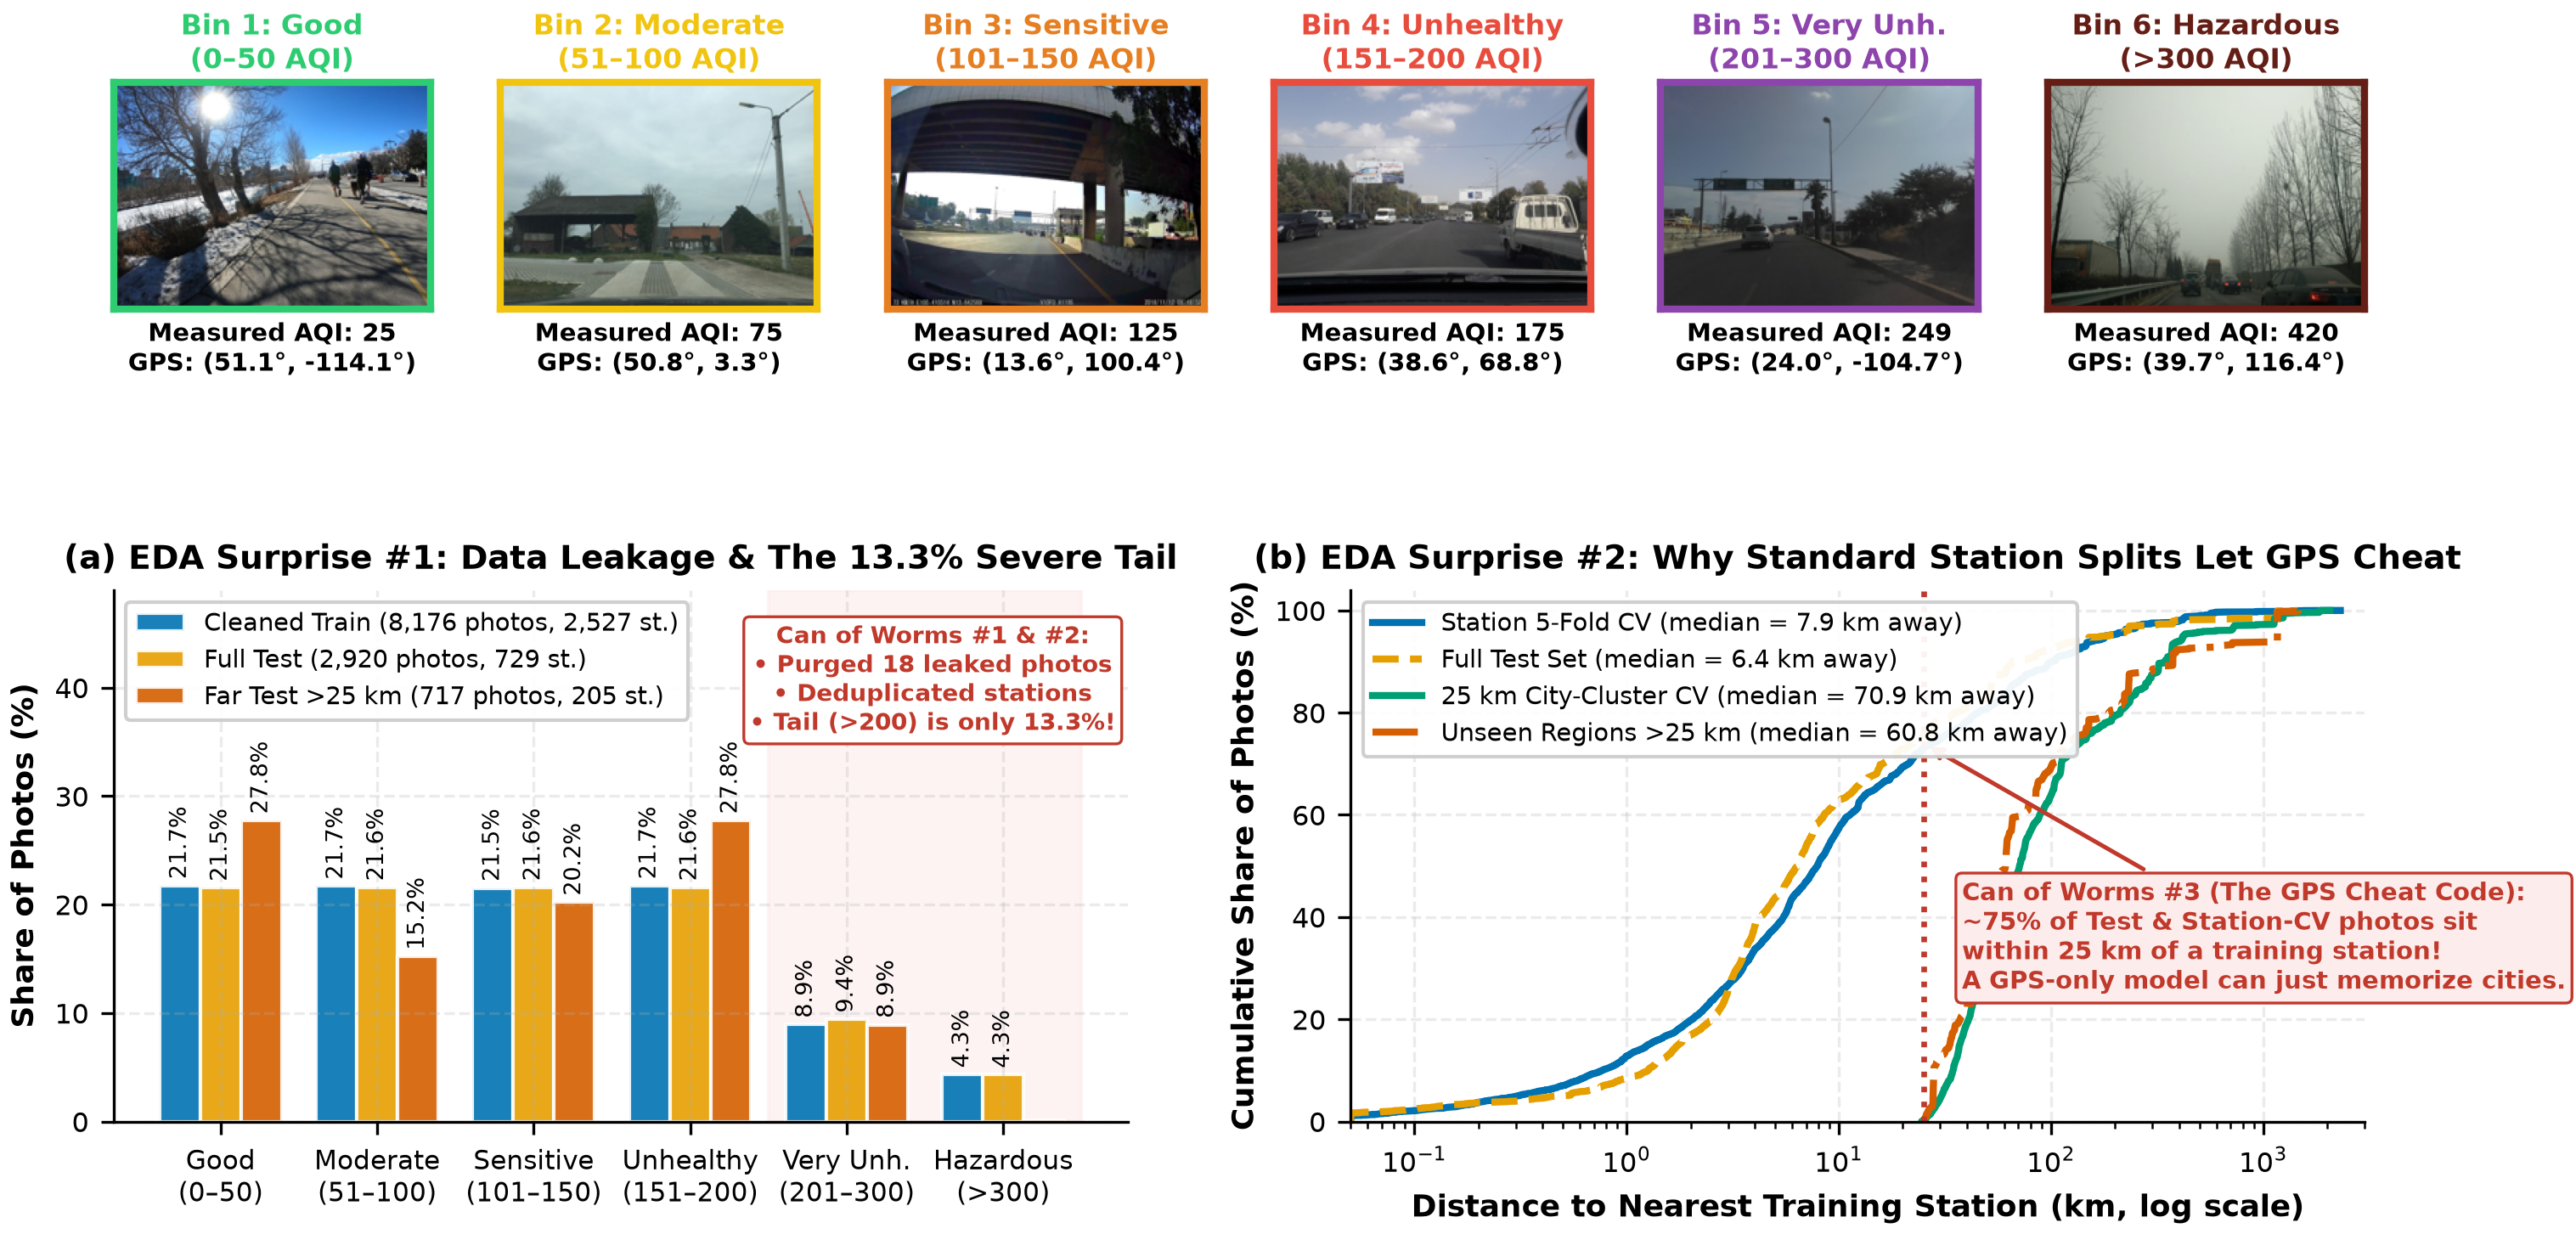
\includegraphics[width=0.98\textwidth]{figures/story_fig1_eda_can_of_worms.png}
  \caption{
    Opening the PM25Vision can of worms during EDA. \textbf{Top row:} Six real
    training photos across the six US EPA AQI bins, showing how camera quality,
    weather, and street scenes vary globally. \textbf{Panel (a):} Class balance
    across our cleaned splits (balanced 0--200 AQI bins at $\sim 21.7\%$ each
    vs.\
    the 13.3\% severe-smog tail above 200 AQI). \textbf{Panel (b):} Distance
    from each validation or test photo to the nearest training station, showing
    that $\sim 75\%$ of standard test and station-CV photos sit within 25~km of
    a training site.
  }
  \label{fig:story_eda}
\end{figure*}

Raw PM25Vision (from Hugging Face, DeadCardassian/PM25Vision) contains 8,298
training rows (8,194 unique image IDs, 2,532 stations) and 2,921 test rows
(2,920 unique image IDs, 729 stations). Our EDA uncovered four major issues
(Fig.~\ref{fig:story_eda}):

\begin{enumerate}
  \item \textbf{Worm \#1 -- The target is US EPA AQI (1--530):} Although the CSV
        column is called \texttt{pm25}, its values span 1.0 to 530.0 and follow
        the exact thresholds (50, 100, 150, 200, 300) of the 6-category
        \textbf{US EPA AQI} scale. We report all errors in native AQI points (in
        training, targets are divided by 100.0 for stable gradients and
        multiplied back by 100.0 before scoring).
  \item \textbf{Worm \#2 -- 18 leaked test images and duplicate rows:} We found
        18 identical image IDs present in both train and test, plus duplicate
        rows matching the same photo to different nearby stations with slightly
        different AQI readings. Our deterministic cleaning script
        (\texttt{cleaning.py}) deletes all 18 overlapping images from train
        (leaving zero shared images or stations between train and test), sorts
        by image and station ID, collapses duplicate rows for the same photo
        using the \textbf{median AQI}, retains the first primary station ID, and
        recomputes the 6-class bin. This yields \textbf{8,176 cleaned training
        photos across 2,527 stations} (mean AQI $121.80 \pm 88.35$, median
        $111.00$) and \textbf{2,920 cleaned test photos across 729 stations}.
  \item \textbf{Worm \#3 -- The 13.3\% severe-smog tail and ``Monster'' Fold~3:}
        As shown in Fig.~\ref{fig:story_eda}(a), the first four AQI buckets
        (0--200) are evenly balanced at $\sim 21.7\%$ each (1,760--1,778 photos
        per bin), whereas severe smog above 200 AQI forms a small 13.28\% tail:
        Bin~5 (\textit{Very Unhealthy}, 731 photos, 8.94\%) and Bin~6
        (\textit{Hazardous}, 355 photos, 4.34\%). Because all photos from a
        station must stay in the same cross-validation fold, \textbf{Fold~3}
        inherited several heavily polluted stations: just four
        $1^\circ \times 1^\circ$ map grid cells (7 stations) in Delhi/NCR
        (34.50\% of Fold~3's tail, mean AQI 288.84), Saltillo/Monterrey
        (20.52\%, mean AQI 474.00), Chiang Rai (13.54\%), and Pune (8.30\%) hold
        \textbf{76.86\% (176 / 229)} of Fold~3's severe-tail images! Fold~3's
        validation AQI standard deviation jumps to 108.20 (vs.\ 79.34--88.38 on
        Folds 0, 1, 2, and 4), causing every model's error to spike by 15--20
        points on Fold~3.
  \item \textbf{Worm \#4 -- The GPS ``Cheat Code'' inside cities:} Computing the
        exact Haversine distance from every validation and test photo to the
        closest training station (Fig.~\ref{fig:story_eda}(b)) revealed that the
        median distance is just \textbf{7.9~km in station CV and 6.4~km in the
        full test set}, with $\sim 75\%$ of photos sitting within 25~km of a
        training station. A model given GPS and month can guess AQI simply by
        memorizing city averages.
\end{enumerate}

To keep our evaluation honest, we never use random image splits. Instead, we use
5-fold Stratified Group $K$-Fold under two grouping rules, plus an unseen-region
test split:
\begin{itemize}
  \item \textbf{5-Fold Station CV (\texttt{station}, 2,527 groups):} All photos
        from the same station stay in one fold. Used for all image-only models.
  \item \textbf{5-Fold 25~km City-Cluster CV (\texttt{spatial\_cluster}, 1,059
        groups):} Links any stations within 25.0~km of each other into one
        connected city cluster (pushing the median nearest-training-station
        distance to 70.9~km). Used to evaluate multimodal fusion without
        same-city GPS leakage.
  \item \textbf{Unseen-Region Test Subset (\texttt{test\_gt25km}):} All 717 test
        photos (across 205 stations) located $> 25.0$~km from any training
        station (median distance 60.8~km).
\end{itemize}

\subsection{Physics-Safe Preprocessing and Honest Last-Epoch Scoring}
\label{subsec:preprocessing_and_scoring}

Standard image-classification tricks like random color jitter (randomly shifting
brightness, contrast, and saturation) and random cropping destroy the
atmospheric haze signal we want to measure~\cite{wangLightweightAirQuality2024,
bylerLocationGeneralizabilityImageBased2025}. We therefore resize every full
photograph directly to $224 \times 224$ pixels (preserving both sky and ground),
ban color jitter and grayscale, and apply only horizontal flips and mild
$\pm 5^\circ$ affine rotations during training.

We score every model on 10 metrics: continuous regression \textbf{MAE} (our main
metric), RMSE, PLCC, SRCC, $R^2$, and the \textbf{Skill Score} relative to the
blind median guess ($\text{MAE}_{\text{median}}$):
\begin{equation}
  \text{Skill}
  = 1 - \frac{\text{MAE}}{\text{MAE}_{\text{median}}}, \label{eq:skill}
\end{equation}
plus 6-bucket classification accuracy (Acc), within-one-bucket accuracy
($\pm 1\text{Acc}$), Macro-F1, and severe-smog tail metrics (\textbf{TailMAE}
and \textbf{TailF1} on Bins 5--6, AQI $> 200$).

Crucially, \textbf{all tables report the final epoch of the fixed training
schedule}. In our failure diagnostics, we discovered that in multitask PFRML
runs, validation loss reaches a false minimum at epochs 2--6 and then rises up
to epoch~30 because the 6-class classifier becomes overconfident on unseen
stations, even while continuous validation MAE keeps improving! Moreover, when
training a final model once on 100\% of the training set for one-shot test
evaluation, no validation split exists to pick a ``best'' epoch. Using the last
epoch everywhere removes checkpoint-selection bias. In 5-fold CV, we report
paired differences $\pm$ standard error ($\text{SE} = \text{SD}/\sqrt{5}$) and
folds won out of 5; on the test set, we compute 95\% confidence intervals via a
\textbf{1,000-resample station-level cluster bootstrap} ($\text{seed} = 42$).

\subsection{Our Model Lineup: From Sanity Checks to PFRML and Fusion}
\label{subsec:model_lineup}

\begin{figure*}[t]
  \centering
  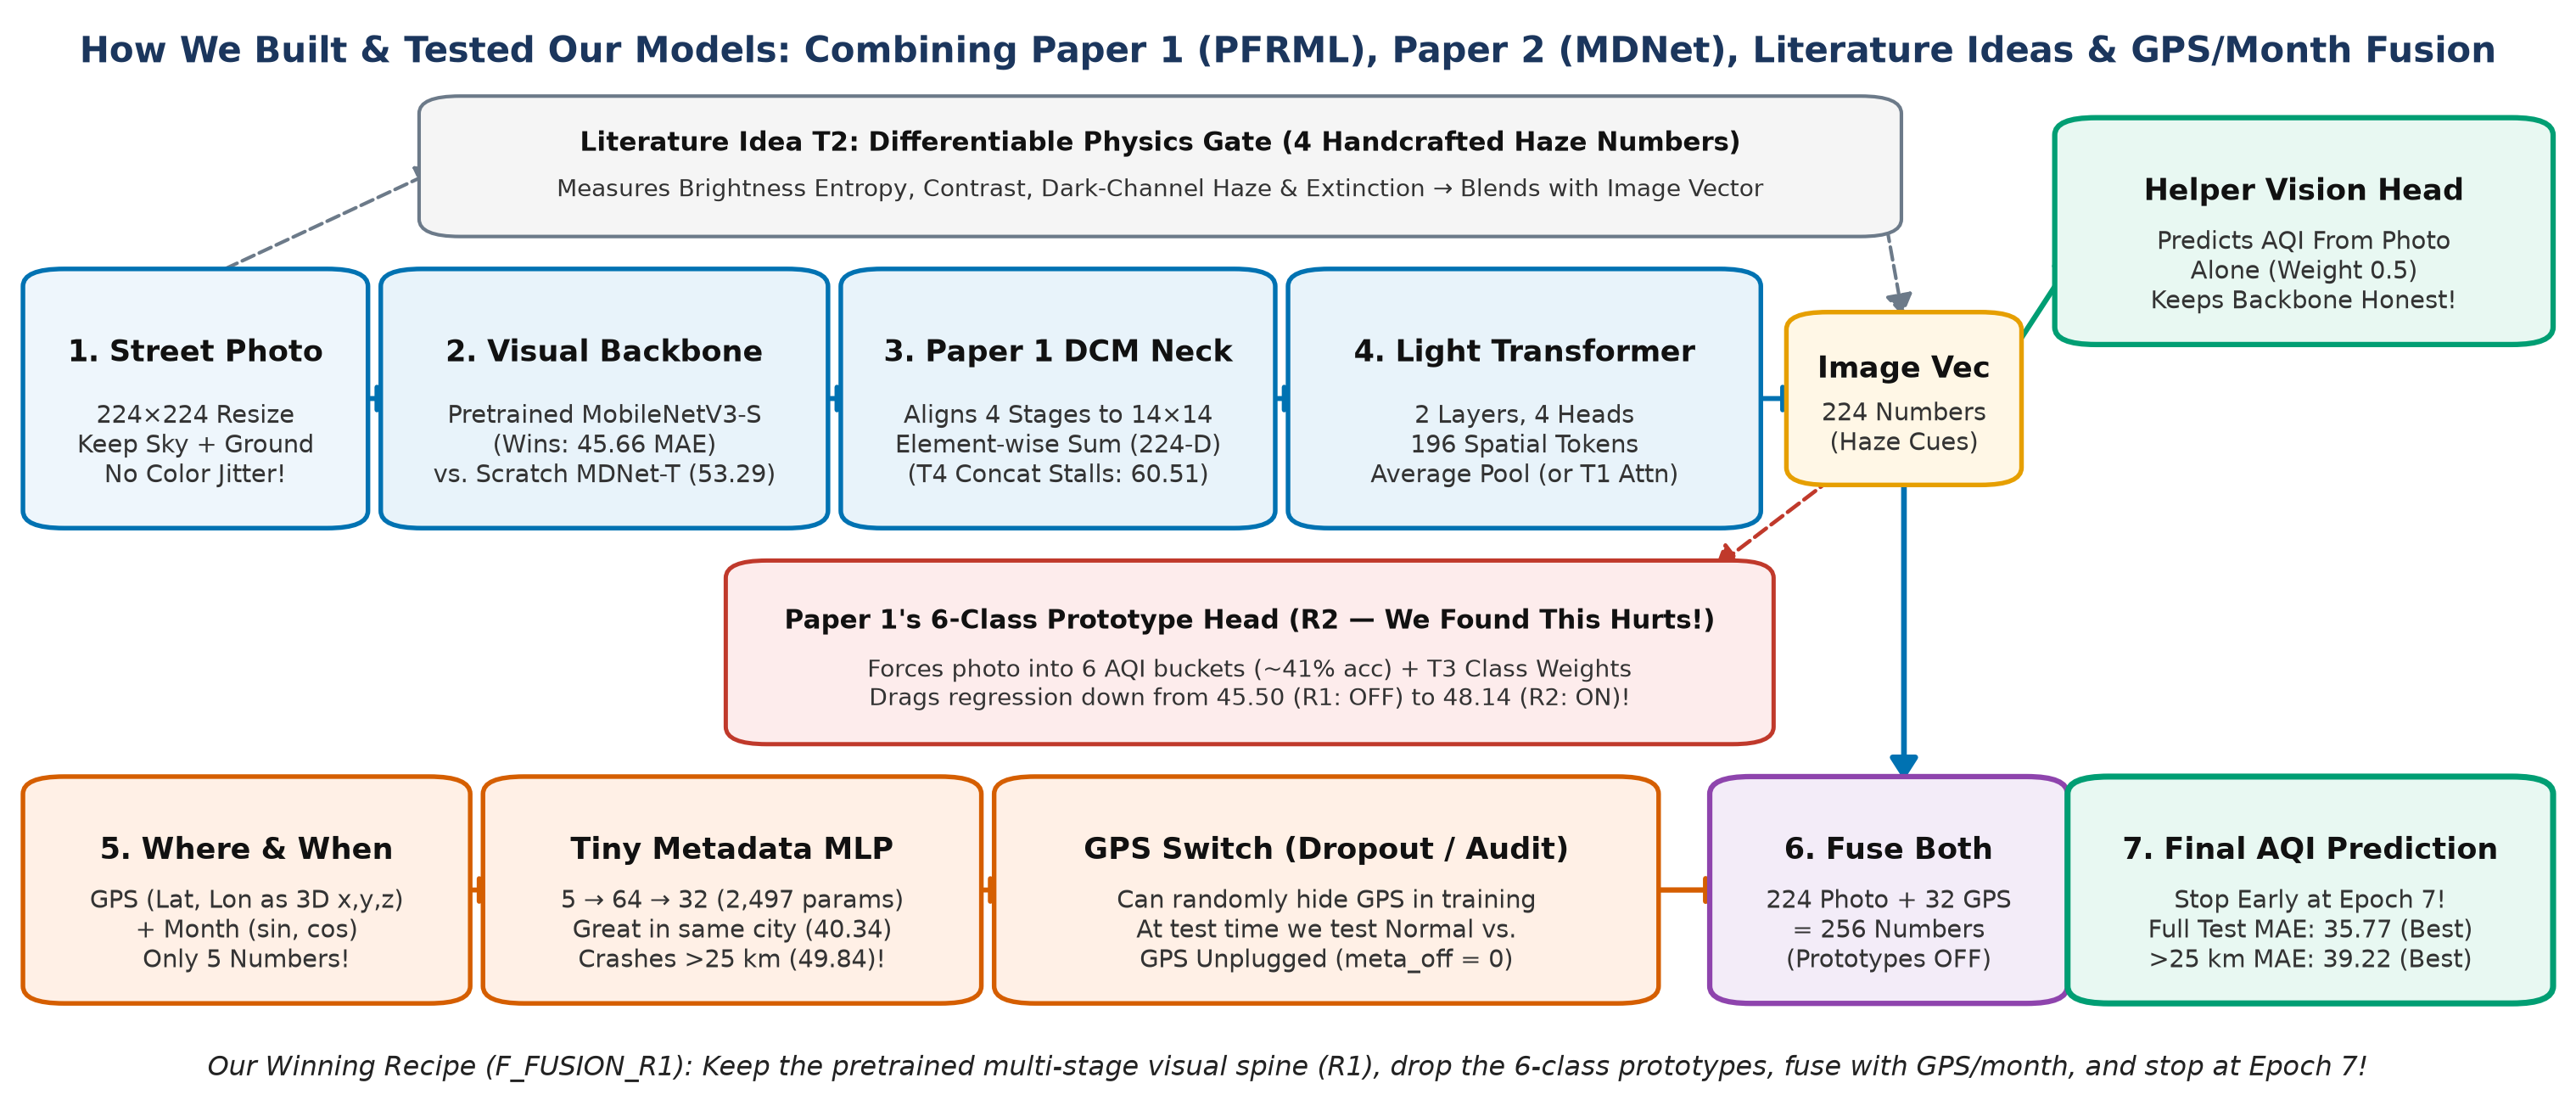
\includegraphics[width=0.98\textwidth]{figures/story_fig2_two_papers_and_pivot.png}
  \caption{
    How we combined Paper~1 (PFRML), Paper~2 (MDNet), and literature add-ons,
    and how our ablation detective work led to our final winning architecture
    (\texttt{F\_FUSION\_R1}): keeping the multi-stage visual spine (Steps 1--4)
    with prototypes turned \textbf{off} (R1), fusing with the 32-number
    GPS/month vector (Steps 5--6), supervising vision with a helper head, and
    stopping early at Epoch~7.
  }
  \label{fig:story_arch}
\end{figure*}

Fig.~\ref{fig:story_arch} illustrates our four progressive model groups:

\subsubsection{Group 1 -- Sanity Checks and the GPS Cheat Detector (E0, E1)}

\begin{itemize}
  \item \textbf{Blind Median Guess (\texttt{E0\_median}):} Always predicts the
        training median ($\sim 111$ AQI), setting our zero-skill floor (66.21
        MAE in station CV).
  \item \textbf{18 Handcrafted Haze Numbers + Ridge (\texttt{E0\_ridge}):}
        Computes mean and standard deviation of HSV color saturation, Sobel edge
        contrast, and the $15 \times 15$ Dark Channel Prior across the full
        photo, top sky half, and bottom ground half (18 features) and fits
        standardized Ridge regression~\cite{marzaguiReviewImageQuality2024,
        chakrabortyCanImageTell2024}.
  \item \textbf{5-Input GPS + Month Network (\texttt{E1\_metadata\_mlp}):} Never
        looks at the photo. Converts latitude and longitude to 3D unit-sphere
        coordinates $(x, y, z)$ and month $m$ to
        $(\sin(2\pi m/12), \cos(2\pi m/12))$, passing those 5 numbers through a
        tiny 2-layer ReLU MLP ($5 \to 64 \to 32 \to 1$; 2,497 parameters, 40
        epochs).
\end{itemize}

\subsubsection{
  Group 2 -- Image-Only Backbones and Our MobileNet + MD-Neck Mashup (E2, E3,
  E3b)
}

\begin{itemize}
  \item \textbf{Standard CNNs From Scratch vs.\ Pretrained (E2):} Compares
        ResNet-18 (11.18M parameters) from random weights (30 epochs) vs.\
        ImageNet-pretrained weights (40 epochs, $\text{lr} = 3 \times 10^{-4}$),
        alongside pretrained MobileNetV3-Small (1.52M parameters, 30 epochs,
        $\text{lr} = 10^{-3}$).
  \item \textbf{Paper~2's MDNet-T From Scratch (E3):} Implements the 4-stage
        MDNet-T CNN~\cite{wangLightweightAirQuality2024} (4.93M parameters, 18
        MDBlocks with parallel dilated depthwise branches at windows
        $5 \times 5$, $3 \times 3$, and $1 \times 1$, yielding a 1,136-pixel
        receptive field), trained from scratch for 60 epochs.
  \item \textbf{Our Lightweight MobileNet + MD-Neck Mashup (E3b):} Because no
        pretrained ImageNet weights exist for MDNet-T, we created our own
        1.04M-parameter hybrid (\texttt{E3b}, not from Paper~2): we take the
        $7 \times 7$ features from pretrained MobileNetV3-Small, reduce channels
        ($576 \to 128$), and pass them through 2 dilated MDBlocks (40 epochs).
\end{itemize}

\subsubsection{
  Group 3 -- Peeling Apart Paper~1 (PFRML) and Literature Add-Ons (E4, E5)
}

To run fair 5-fold ablations on our laptop GPU, we pair
PFRML~\cite{wangPrototypeFeatureRepresentationGuided2026} with our pretrained
MobileNetV3-Small backbone ($\sim 2.0\text{M}$ parameters, 30 epochs at
$\text{lr} = 10^{-3}$) as well as from-scratch MDNet-T:
\begin{enumerate}
  \item \textbf{Multi-Stage DCM + Light Transformer Spine:} The Dimension
        Consistency Module (DCM) taps four backbone stages ($56 \times 56$ down
        to $7 \times 7$), projects each to 224 channels, aligns them to
        $14 \times 14$, and sums them. A 2-layer Light Transformer (4 heads)
        processes the 196 spatial patches + \texttt{[CLS]} with 2D positional
        embeddings and pools them into a 224-number visual vector $\chi_i$.
  \item \textbf{The 6-Class Prototype Head (R1 vs.\ R2 vs.\ Eq.~5):} Paper~1
        maintains 6 unit-sphere reference vectors (prototypes) $\{p_k\}_{k=0}^5$
        updated by Exponential Moving Average (EMA) and classifies each photo by
        squared Euclidean distance:
        \begin{equation}
          P(y = k \mid \chi_i) = \frac{\exp\!\big( -\|\hat{\chi}_i - \hat{p}_k\|_2^2 / \tau \big)}{\sum_{j=0}^{5} \exp\!\big( -\|\hat{\chi}_i - \hat{p}_j\|_2^2 / \tau \big)}. \label{eq:proto_softmax}
        \end{equation}
        Because Paper~1's Eq.~5 feeds only $\chi_i$ to the regression MLP while
        its Fig.~7 concatenates the prototype-weighted vector
        $\tilde{c}_i = \sum_k P(y = k \mid \chi_i)\hat{p}_k$, we test all three
        rungs: \textbf{Rung~R1} (prototypes completely OFF, pure MSE on
        $\chi_i$), \textbf{Rung~R2} (prototypes ON, regression reads
        $[\chi_i; \tilde{c}_i]$), and \textbf{Rung~R2 Eq.~5} (prototypes ON,
        regression reads $\chi_i$ only).
  \item \textbf{Four Literature Add-Ons (T1--T4):} Onto R2, we test \textbf{T1}
        learned spatial token attention
        pooling~\cite{abdelsalamSkyFuseNetCrossAttentionSwin2026,
        leeEnhancingPM25Detection2025}, \textbf{T2} a differentiable 4-scalar
        physics gate (luminance entropy, contrast, dark-channel transmission
        $t$, and extinction $-\ln(t)$)~\cite{dohaDeepMultiTaskLearning2026,
        yadavRoadsideTreeImageBased2025}, \textbf{T3} inverse-frequency class
        weights ($N_k^{-0.5}$) for the rare severe-smog
        tail~\cite{dohaDeepMultiTaskLearning2026,
        bylerLocationGeneralizabilityImageBased2025}, \textbf{T4} DCM stage
        concatenation ($896 \to 224$) instead of addition, and \textbf{R2+all}
        (combining T1+T2+T3 with sum DCM).
\end{enumerate}

\subsubsection{Group 4 -- Multimodal Fusion and Epoch-7 Early Stopping (E5)}

Our Fusion network concatenates the 224-number visual vector $\chi_i$ with the
32-number GPS/month embedding $m_i$ into a shared regression MLP
($256 \to 256 \to 1$). To prevent the fast-learning GPS branch from dominating
the camera backbone, we train under 5-fold 25~km city-cluster CV with: (1) a
detached \textbf{Helper Vision Head} ($224 \to 256 \to 1$) weighted by
$\lambda_{\text{aux}} = 0.5$ in the total loss:
\begin{equation}
  \mathcal{L}
  = \mathcal{L}_{\text{cls}}
    + \beta\,\mathcal{L}_{\text{reg}}
    + \lambda_{\text{aux}}\,\mathcal{L}_{\text{aux}}, \label{eq:total_loss}
\end{equation}
(2) per-sample GPS modality dropout ($p_{\text{drop}} \in \{0.3, 0.0\}$) plus an
\textbf{unplugged-GPS test audit} (\texttt{meta\_off}, setting $m_i = 0$ at test
time), and (3) \textbf{CMA-3 early stopping at $N = 7$ epochs}, selected where
the 3-epoch moving average of 25~km city-cluster validation MAE hit its minimum
(46.26 CMA-3, 45.74 raw MAE) before city-coordinate overfitting began.

\section{Results}
\label{sec:results}

\subsection{
  Act 1 -- The Wake-Up Call: Simple Haze Formulas Fail, and a Tiny GPS Network
  Beats Our Pixels
}
\label{subsec:act1_baselines}

\begin{table*}[t]
  \centering
  \caption{
    Act 1 Sanity Checks: Non-Visual and Handcrafted Haze Baselines Across 5-Fold
    Station CV ($n = 8,176$), 5-Fold 25~km City-Cluster CV ($n = 8,176$), Full
    Test Set ($n = 2,920$, 729 Stations), and Unseen Regions $> 25$~km Away
    ($n = 717$, 205 Stations).
  }
  \label{tab:story_baselines}
  \footnotesize
  \setlength{\tabcolsep}{4.5pt}
  \resizebox{\textwidth}{!}{%
    \begin{tabular}{llccccccccccc}
      \toprule
      \textbf{Baseline Model (ID)}                 & \textbf{Evaluation Split} & $\boldsymbol{n}$ & \textbf{MAE (Mean $\pm$ SD / [95\% CI])} & \textbf{RMSE} & \textbf{PLCC} & \textbf{SRCC} & $\boldsymbol{R^2}$ & \textbf{Acc} & $\boldsymbol{\pm 1}$\textbf{Acc} & \textbf{MacroF1} & \textbf{TailMAE} & \textbf{TailF1} \\
      \midrule
      Blind Median Guess (\texttt{E0\_median})     & Station 5-fold CV         &       8176       &             $66.21 \pm 4.89$             &    $88.23$    &   $0.0000$    &   $0.0000$    &     $-0.0161$      &   $0.2153$   &             $0.6497$             &     $0.0590$     &     $176.95$     &    $0.0000$     \\
      Blind Median Guess (\texttt{E0\_median})     & 25~km City-Cluster CV     &       8176       &             $66.14 \pm 5.60$             &    $88.00$    &   $0.0000$    &   $0.0000$    &     $-0.0168$      &   $0.2154$   &             $0.6500$             &     $0.0591$     &     $175.81$     &    $0.0000$     \\
      Blind Median Guess (\texttt{E0\_median})     & Full Test Set             &       2920       &                 $63.64$                  &    $81.88$    &   $0.0000$    &   $0.0000$    &     $-0.0105$      &   $0.2158$   &             $0.6473$             &     $0.0592$     &     $155.88$     &    $0.0000$     \\
      Blind Median Guess (\texttt{E0\_median})     & Unseen $> 25$~km Test     &       717        &                 $56.60$                  &    $64.22$    &   $0.0000$    &   $0.0000$    &     $-0.0049$      &   $0.2022$   &             $0.6318$             &     $0.0561$     &     $102.78$     &    $0.0000$     \\
      \midrule
      18 Haze Numbers Ridge (\texttt{E0\_ridge})   & Station 5-fold CV         &       8176       &             $64.11 \pm 4.40$             &    $86.32$    &   $0.1998$    &   $0.2354$    &      $0.0301$      &   $0.2450$   &             $0.6925$             &     $0.1330$     &     $158.15$     &    $0.0000$     \\
      18 Haze Numbers Ridge (\texttt{E0\_ridge})   & 25~km City-Cluster CV     &       8176       &             $64.56 \pm 5.02$             &    $87.37$    &   $0.1526$    &   $0.1982$    &     $-0.0018$      &   $0.2415$   &             $0.6915$             &     $0.1325$     &     $160.68$     &    $0.0000$     \\
      18 Haze Numbers Ridge (\texttt{E0\_ridge})   & Full Test Set             &       2920       &                 $60.84$                  &    $79.77$    &   $0.2112$    &   $0.2258$    &      $0.0408$      &   $0.2250$   &             $0.6815$             &     $0.1109$     &     $140.91$     &    $0.0000$     \\
      18 Haze Numbers Ridge (\texttt{E0\_ridge})   & Unseen $> 25$~km Test     &       717        &                 $53.76$                  &    $65.26$    &   $0.1435$    &   $0.0970$    &     $-0.0377$      &   $0.2092$   &             $0.6792$             &     $0.1142$     &     $107.93$     &    $0.0000$     \\
      \midrule
      GPS + Month MLP (\texttt{E1\_metadata\_mlp}) & Station 5-fold CV         &       8176       &        $\mathbf{43.15 \pm 7.47}$         &    $65.43$    &   $0.6704$    &   $0.7260$    &      $0.4438$      &   $0.4234$   &             $0.8794$             &     $0.3506$     &     $104.96$     &    $0.1632$     \\
      GPS + Month MLP (\texttt{E1\_metadata\_mlp}) & 25~km City-Cluster CV     &       8176       &        $\mathbf{46.00 \pm 7.33}$         &    $70.09$    &   $0.6257$    &   $0.7147$    &      $0.3647$      &   $0.4183$   &             $0.8603$             &     $0.3556$     &     $118.49$     &    $0.1953$     \\
      GPS + Month MLP (\texttt{E1\_metadata\_mlp}) & Full Test Set             &       2920       &     $\mathbf{40.34}\;[34.45, 48.31]$     &    $57.70$    &   $0.7098$    &   $0.7344$    &      $0.4982$      &   $0.4096$   &             $0.8873$             &     $0.3397$     &     $76.82$      &    $0.1362$     \\
      GPS + Month MLP (\texttt{E1\_metadata\_mlp}) & Unseen $> 25$~km Test     &       717        &     $\mathbf{49.84}\;[40.18, 58.81]$     &    $65.31$    &   $0.3797$    &   $0.4954$    & $\mathbf{-0.0393}$ &   $0.2929$   &             $0.7476$             &     $0.2004$     &     $88.83$      &    $0.0000$     \\
      \bottomrule
    \end{tabular}%
  }
\end{table*}

Table~\ref{tab:story_baselines} answers Question~1 with two immediate lessons.
First, our 18 handcrafted haze features (\texttt{E0\_ridge}) barely improve over
blindly guessing the median ($64.11$ vs.\ $66.21$ MAE in station CV,
$R^2 = 0.0301$). When photos come from thousands of different street cameras and
weather conditions, simple global averages of saturation, contrast, and the Dark
Channel Prior cannot separate overcast skies from actual pollution.

Second, our tiny 5-input GPS-and-month neural network (\texttt{E1}) gets
\textbf{43.15 $\pm$ 7.47 MAE} in station CV and \textbf{40.34 MAE
($R^2 = 0.4982$)} on the full test set \textit{without looking at a single image
pixel}! Because 75\% of test photos sit in the same cities as training stations,
memorizing city locations and seasons looks deceptively accurate. However, on
the 717 test photos located $> 25$~km from any training station, the GPS-only
model jumps by $+9.50$ points to \textbf{49.84 MAE} and its explained variance
crashes to \textbf{$R^2 = -0.0393$} (worse than predicting a constant average).

\subsection{
  Act 2 -- When Our First Fancy Model Flopped, ImageNet Pretraining Saved Vision
}
\label{subsec:act2_backbones}

\begin{table*}[t]
  \centering
  \caption{
    Act 2 Vision-Only Showdown Under 5-Fold Station-Grouped Cross-Validation
    ($n = 8,176$, Last-Epoch Metrics). Skill Measures Error Reduction Relative
    to the Blind Median Guess (66.21 MAE).
  }
  \label{tab:story_backbones}
  \footnotesize
  \setlength{\tabcolsep}{4pt}
  \resizebox{\textwidth}{!}{%
    \begin{tabular}{llcccccccccccc}
      \toprule
      \textbf{Vision Model (ID)}                 & \textbf{Size / Training Schedule} &   \textbf{Last-Ep MAE}    &   \textbf{Skill}   &  \textbf{F0 / F1 / F2 / F3 / F4 MAE}  &  \textbf{RMSE}   &   \textbf{PLCC}   &   \textbf{SRCC}   & $\boldsymbol{R^2}$ &   \textbf{Acc}    & $\boldsymbol{\pm 1}$\textbf{Acc} & \textbf{MacroF1}  & \textbf{TailMAE}  &  \textbf{TailF1}  \\
      \midrule
      Pretrained ResNet-18 (\texttt{E2})         & 11.18M (lr 3e-4, 40ep)            & $\mathbf{44.05 \pm 8.70}$ & $\mathbf{+0.3346}$ & 34.85 / 43.35 / 42.06 / 58.45 / 41.55 & $\mathbf{68.22}$ & $\mathbf{0.6441}$ & $\mathbf{0.7060}$ & $\mathbf{0.3862}$  &     $0.4102$      &        $\mathbf{0.8656}$         &     $0.3751$      & $\mathbf{116.26}$ &     $0.2822$      \\
      Our MobileNetV3-S + MD-Neck (\texttt{E3b}) & 1.04M (lr 1e-3, 40ep)             & $\mathbf{44.92 \pm 8.54}$ &     $+0.3214$      & 34.51 / 45.40 / 43.31 / 58.25 / 43.14 &     $70.23$      &     $0.6173$      &     $0.6780$      &      $0.3461$      & $\mathbf{0.4137}$ &             $0.8482$             & $\mathbf{0.3789}$ &     $118.93$      &     $0.2913$      \\
      Pretrained MobileNetV3-Small (\texttt{E2}) & 1.52M (lr 1e-3, 30ep)             & $\mathbf{45.66 \pm 8.41}$ &     $+0.3103$      & 36.27 / 46.10 / 42.96 / 59.21 / 43.77 &     $70.41$      &     $0.6152$      &     $0.6695$      &      $0.3450$      &     $0.4044$      &             $0.8488$             &     $0.3776$      &     $119.16$      & $\mathbf{0.3135}$ \\
      \midrule
      From-Scratch ResNet-18 (\texttt{E2})       & 11.18M (lr 1e-3, 30ep)            &     $53.27 \pm 7.11$      &     $+0.1954$      & 48.41 / 50.21 / 53.62 / 65.44 / 48.67 &     $76.77$      &     $0.5177$      &     $0.5367$      &      $0.2314$      &     $0.3276$      &             $0.7943$             &     $0.2975$      &     $126.93$      &     $0.2302$      \\
      Paper 2 MDNet-T From Scratch (\texttt{E3}) & 4.93M (lr 1e-3, 60ep)             &     $53.29 \pm 6.38$      &     $+0.1951$      & 48.37 / 50.74 / 53.97 / 64.06 / 49.31 &     $77.16$      &     $0.5260$      &     $0.5365$      &      $0.2226$      &     $0.3371$      &             $0.7797$             &     $0.3030$      &     $129.51$      &     $0.2175$      \\
      \bottomrule
    \end{tabular}%
  }
\end{table*}

\begin{figure}[t]
  \centering
  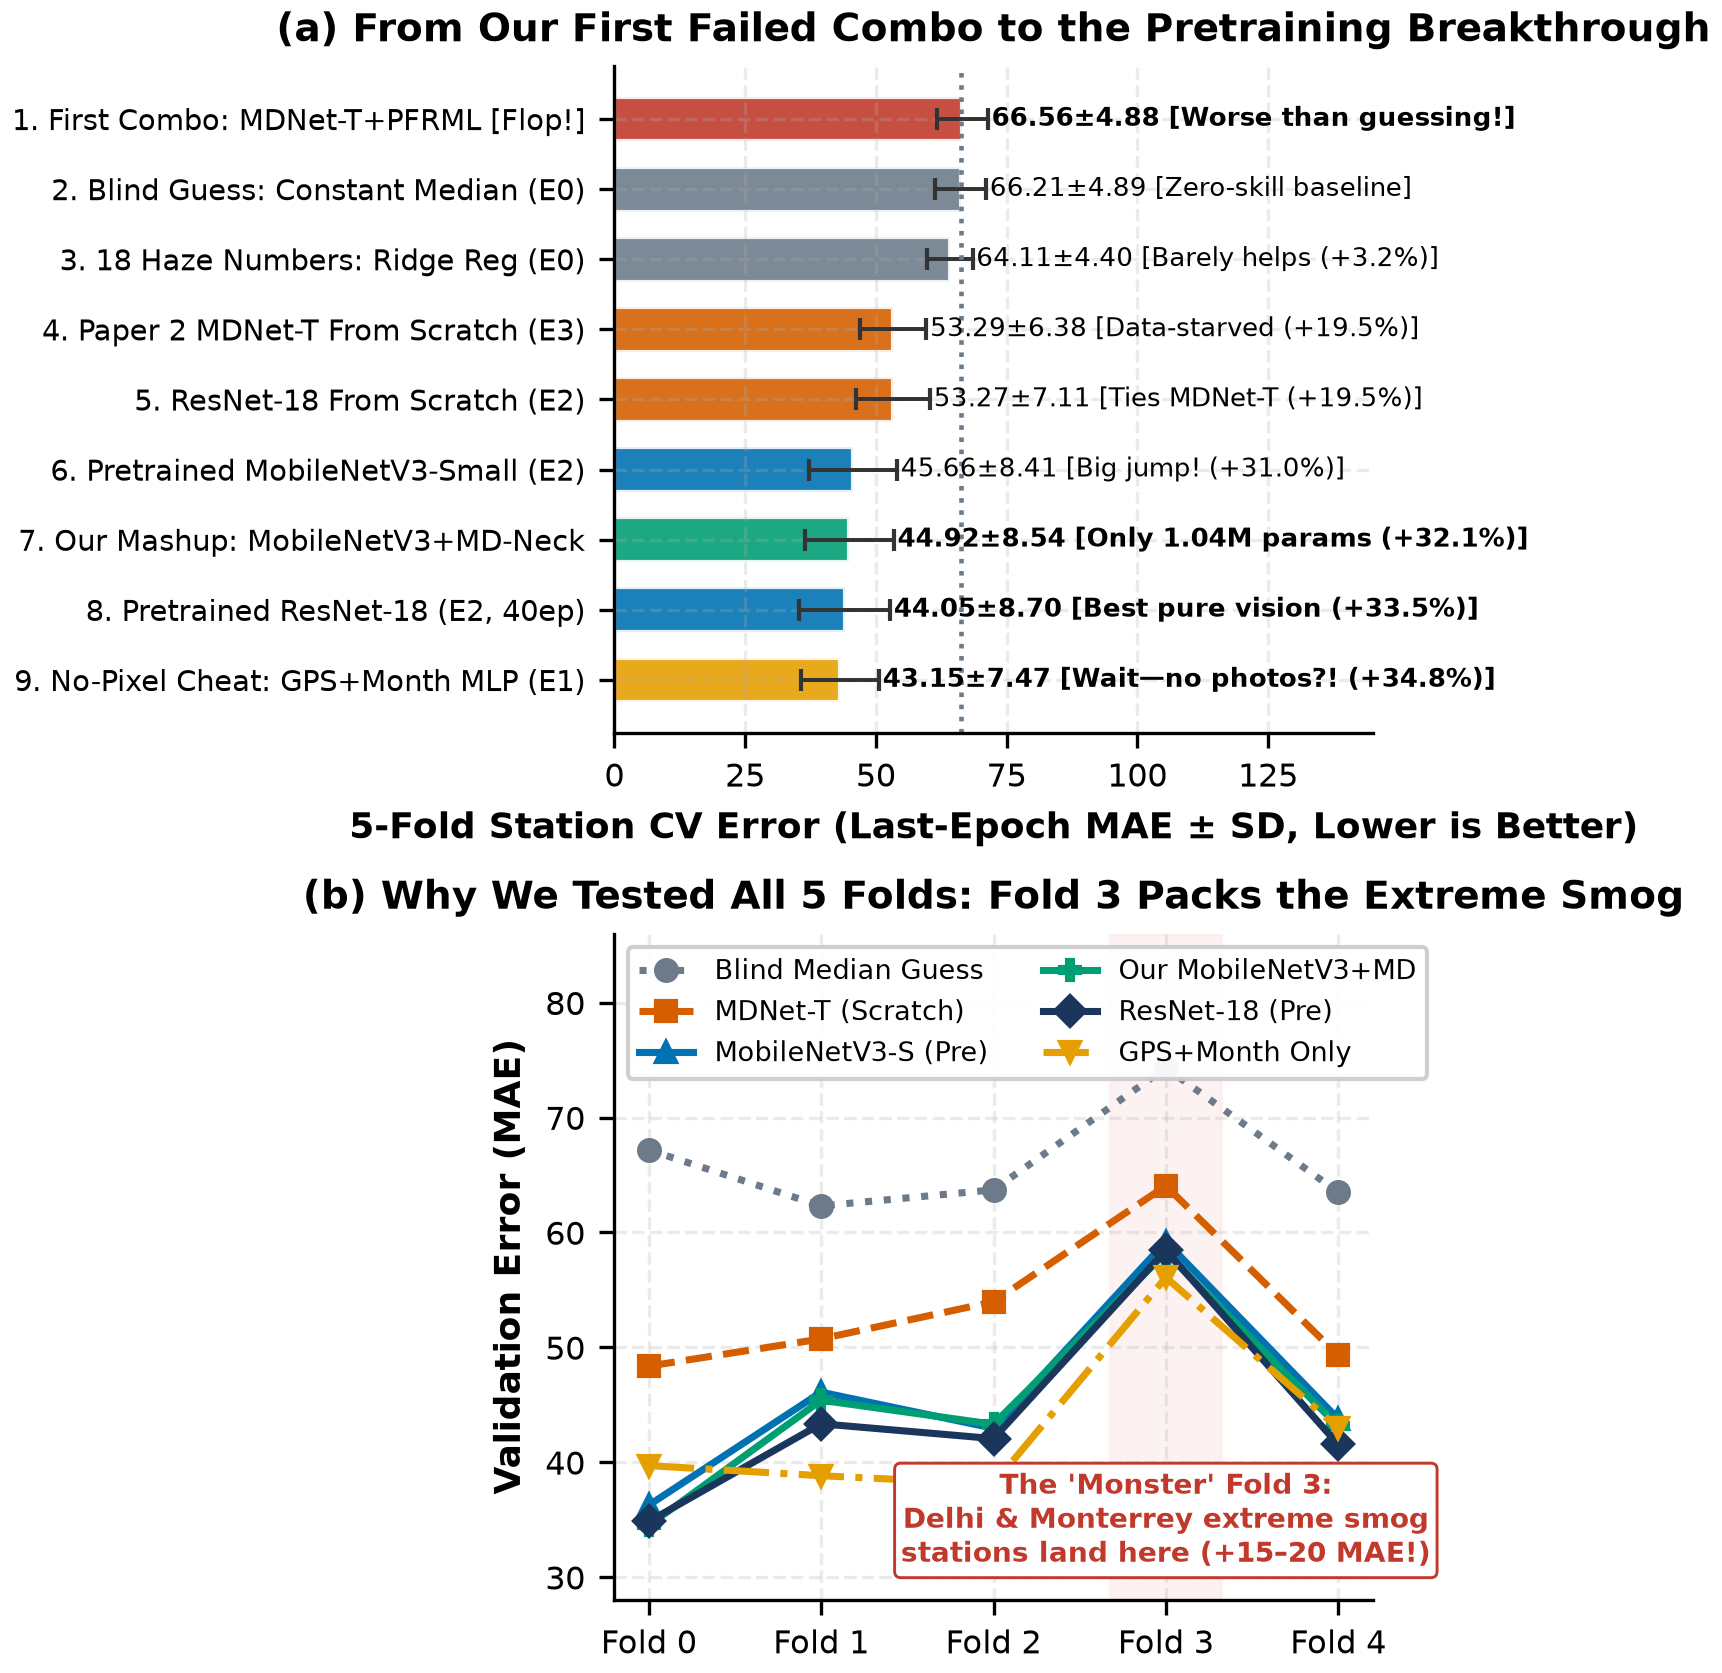
\includegraphics[width=\columnwidth]{figures/story_fig3_first_experiments_to_transfer_win.png}
  \caption{
    \textbf{(a)} Progression from our first failed MDNet-T + PFRML combo (66.56
    MAE) and data-starved from-scratch CNNs ($\sim 53.3$ MAE) to the 8--9 point
    ImageNet pretraining breakthrough ($44.05\text{--}45.66$ MAE). \textbf{(b)}
    Validation MAE across all 5 station folds, highlighting the Fold~3
    severe-smog spike.
  }
  \label{fig:story_backbones}
\end{figure}

Table~\ref{tab:story_backbones} and Fig.~\ref{fig:story_backbones} answer
Question~2. Training Paper~2's custom MDNet-T from scratch for 60 epochs got
\textbf{53.29 $\pm$ 6.38 MAE}---virtually identical to a from-scratch ResNet-18
(\textbf{53.27 $\pm$ 7.11 MAE}). On roughly 6,540 diverse training photos per
fold, a randomly initialized network simply lacks the visual foundation to
separate street geometry from atmospheric haze.

Switching to \textbf{ImageNet-pretrained weights} slashed 5-fold error by 7.61
to 9.24 AQI points across every fold: pretrained ResNet-18 reached \textbf{44.05
$\pm$ 8.70 MAE}, our 1.04M-parameter MobileNetV3-S + MD-Neck mashup
(\texttt{E3b}) reached \textbf{44.92 $\pm$ 8.54 MAE} (achieving the top 6-class
accuracy of 41.37\% among image baselines), and plain pretrained
MobileNetV3-Small reached \textbf{45.66 $\pm$ 8.41 MAE} at $7 \times$ fewer
parameters than ResNet-18.

\subsection{
  Act 3 -- Detective Work on Paper 1: Why PFRML's 6-Class Prototypes Backfired
}
\label{subsec:act3_pfrml}

\begin{table*}[t]
  \centering
  \caption{
    Act 3 Detective Work: Peeling Apart Paper~1 (PFRML) and Literature Add-Ons
    Across All 5 Station-Disjoint Folds ($n = 8,176$, Last-Epoch Metrics).
    Negative Paired Differences Mean the Row Beats the Reference Model.
  }
  \label{tab:story_pfrml}
  \footnotesize
  \setlength{\tabcolsep}{4pt}
  \resizebox{\textwidth}{!}{%
    \begin{tabular}{lccccccccccc}
      \toprule
      \textbf{Ablation Step / What We Changed}                             &   \textbf{Last-Ep MAE}    &   \textbf{Skill}   & \textbf{Diff vs.\ R1 (Won)} & \textbf{Diff vs.\ E2 (Won)} &       \textbf{Diff vs.\ R2 (Won)}        &  \textbf{RMSE}   &   \textbf{SRCC}   & $\boldsymbol{R^2}$ &   \textbf{Acc}    & $\boldsymbol{\pm 1}$\textbf{Acc} & \textbf{TailMAE}  \\
      \midrule
      \textbf{R1:} Keep DCM + Transformer Neck, \textbf{DROP Prototypes}   & $\mathbf{45.50 \pm 8.64}$ & $\mathbf{+0.3127}$ &   $+0.00 \pm 0.00$ (---)    &   $-0.16 \pm 0.36$ (4/5)    & $\mathbf{-2.63 \pm 1.10}$ (\textbf{4/5}) & $\mathbf{71.44}$ & $\mathbf{0.6671}$ & $\mathbf{0.3249}$  &     $0.4080$      &        $\mathbf{0.8448}$         & $\mathbf{115.37}$ \\
      \textbf{R2:} Paper~1 PFRML Default (Prototypes ON, concat)           &     $48.14 \pm 7.61$      &     $+0.2729$      &   $+2.63 \pm 1.10$ (1/5)    &   $+2.47 \pm 0.95$ (1/5)    &          $+0.00 \pm 0.00$ (---)          &     $75.43$      &     $0.6327$      &      $0.2424$      &     $0.4088$      &             $0.8181$             &     $124.19$      \\
      \textbf{R2 Eq.~5:} Prototypes ON (No prototype concat in regression) &     $48.04 \pm 8.20$      &     $+0.2743$      &   $+2.54 \pm 0.42$ (0/5)    &   $+2.38 \pm 0.46$ (0/5)    &          $-0.09 \pm 0.73$ (2/5)          &     $75.14$      &     $0.6406$      &      $0.2538$      &     $0.4025$      &             $0.8182$             &     $123.27$      \\
      \midrule
      \textbf{R2 + T1:} Add Spatial Token Attention Pooling                &     $48.40 \pm 7.74$      &     $+0.2689$      &   $+2.90 \pm 1.01$ (1/5)    &   $+2.74 \pm 0.97$ (1/5)    &          $+0.27 \pm 0.32$ (2/5)          &     $75.42$      &     $0.6352$      &      $0.2429$      &     $0.4032$      &             $0.8148$             &     $121.92$      \\
      \textbf{R2 + T2:} Add 4-Number Atmospheric Physics Gate              &     $47.57 \pm 6.73$      &     $+0.2815$      &   $+2.07 \pm 1.00$ (1/5)    &   $+1.91 \pm 0.78$ (1/5)    &          $-0.57 \pm 0.86$ (4/5)          &     $74.19$      &     $0.6405$      &      $0.2761$      &     $0.4037$      &             $0.8243$             &     $118.49$      \\
      \textbf{R2 + T3:} Add Rare-Class Weights for High Smog               &     $47.06 \pm 8.01$      &     $+0.2892$      &   $+1.55 \pm 0.73$ (1/5)    &   $+1.40 \pm 0.50$ (0/5)    & $\mathbf{-1.08 \pm 0.49}$ (\textbf{4/5}) &     $73.67$      &     $0.6342$      &      $0.2822$      &     $0.4113$      &             $0.8142$             &     $124.33$      \\
      \textbf{R2 + T4:} Concatenate 4 Stages in DCM (\textit{Broke!})      &     $60.51 \pm 5.41$      &     $+0.0860$      &   $+15.01 \pm 3.38$ (0/5)   &   $+14.85 \pm 3.28$ (0/5)   &         $+12.38 \pm 3.49$ (0/5)          &     $85.22$      &     $0.4082$      &      $0.0556$      &     $0.3041$      &             $0.6664$             &     $168.58$      \\
      \textbf{R2 + all:} Combine Prototypes + T1 + T2 + T3 (Sum DCM)       &     $47.16 \pm 7.15$      &     $+0.2878$      &   $+1.65 \pm 0.92$ (2/5)    &   $+1.49 \pm 0.65$ (1/5)    &          $-0.98 \pm 0.90$ (4/5)          &     $74.22$      &     $0.6398$      &      $0.2774$      & $\mathbf{0.4150}$ &             $0.8136$             &     $121.05$      \\
      \midrule
      \textbf{First Combo:} PFRML on From-Scratch MDNet-T (\textit{Flop!}) &     $66.56 \pm 4.88$      &     $-0.0053$      &   $+21.05 \pm 2.97$ (0/5)   &   $+20.90 \pm 2.79$ (0/5)   &         $+18.42 \pm 2.95$ (0/5)          &     $87.26$      &     $0.0817$      &      $0.0054$      &     $0.1489$      &             $0.4432$             &     $166.28$      \\
      \bottomrule
    \end{tabular}%
  }
\end{table*}

\begin{table}[t]
  \centering
  \caption{
    Why Two Models Stalled: Training Loss From Epoch 1 to Final Epoch Across
    5-Fold Station CV.
  }
  \label{tab:story_collapse}
  \footnotesize
  \setlength{\tabcolsep}{3.5pt}
  \resizebox{\columnwidth}{!}{%
    \begin{tabular}{lccccc}
      \toprule
      \textbf{Model Configuration}     & \textbf{Folds} & \textbf{Ep 1 Loss} & \textbf{End Loss} & \textbf{Last MAE} & \textbf{Last $\boldsymbol{R^2}$} \\
      \midrule
      MDNet-T + PFRML (lr 1e-3, 60ep)  &      5/5       &      $2.1609$      &     $2.1784$      & $66.56 \pm 4.88$  &             $0.0054$             \\
      MDNet-T + PFRML (lr 2e-4, F0)    &      1/5       &      $2.2084$      &     $1.9243$      &   $58.15$ (F0)    &             $0.2910$             \\
      R2 + T4: DCM Concat (30ep)       &      5/5       &      $2.0567$      &     $1.9196$      & $60.51 \pm 5.41$  &             $0.0556$             \\
      \midrule
      R2: PFRML Default (Sum DCM)      &      5/5       &      $1.9949$      &     $0.4621$      & $48.14 \pm 7.61$  &             $0.2424$             \\
      MDNet-T Reg Only (lr 1e-3, 60ep) &      5/5       &      $0.8545$      &     $0.0275$      & $53.29 \pm 6.38$  &             $0.2226$             \\
      \bottomrule
    \end{tabular}%
  }
\end{table}

\begin{figure}[t]
  \centering
  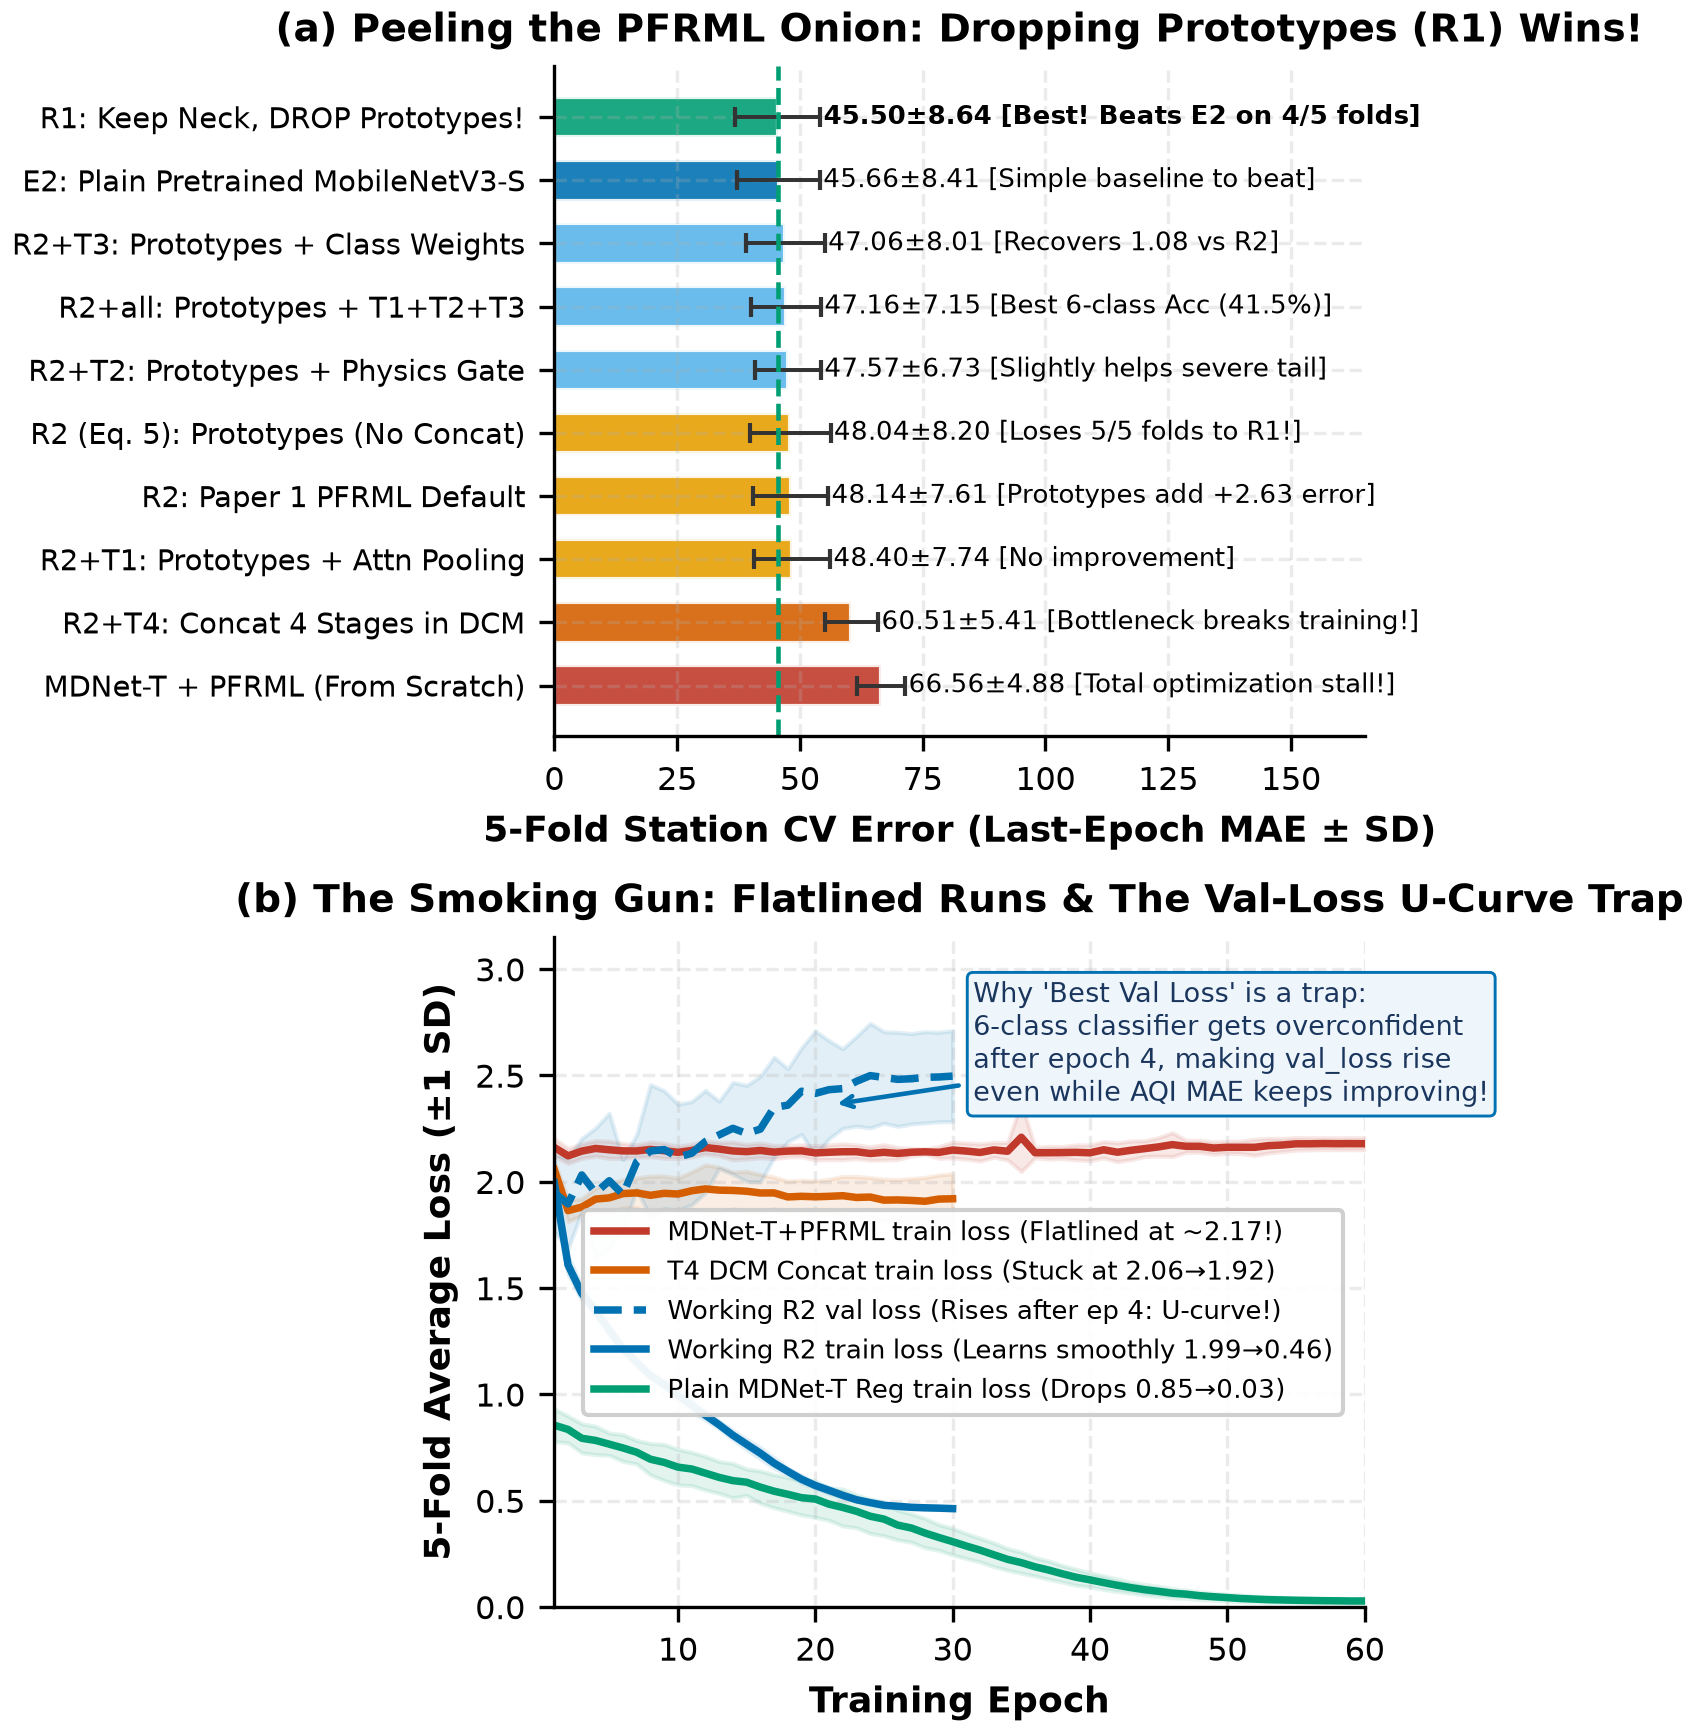
\includegraphics[width=\columnwidth]{figures/story_fig4_why_pfrml_prototypes_backfired.png}
  \caption{
    \textbf{(a)} 5-fold PFRML ablation ladder showing that dropping prototypes
    (R1, 45.50 MAE) beats every prototype variant. \textbf{(b)} Training and
    validation loss curves showing flatlined optimization in MDNet-T+PFRML and
    T4 DCM Concat alongside the validation-loss U-curve in R2.
  }
  \label{fig:story_pfrml}
\end{figure}

Tables~\ref{tab:story_pfrml}--\ref{tab:story_collapse} and
Fig.~\ref{fig:story_pfrml} solve Question~3:
\begin{enumerate}
  \item \textbf{Dropping prototypes (R1) wins:} Keeping Paper~1's 4-stage DCM
        and Light Transformer neck without prototypes (R1) achieves
        \textbf{45.50 $\pm$ 8.64 MAE}, edging out plain MobileNetV3-Small
        ($45.66 \pm 8.41$) on 4/5 folds and lowering severe-smog TailMAE to
        115.37.
  \item \textbf{Turning ON the 6-class prototypes (R2 and Eq.~5) hurts
        regression by 2.5--2.6 MAE points:} Enabling prototypes worsens MAE to
        \textbf{48.14 $\pm$ 7.61} in R2 and \textbf{48.04 $\pm$ 8.20} in literal
        Eq.~5 (which loses 5/5 folds to R1). As the dashed blue curve in
        Fig.~\ref{fig:story_pfrml}(b) reveals, 6-class accuracy across diverse
        global cameras plateaus near $\sim 41\%$, causing the cross-entropy loss
        to become overconfident after epoch~4 and compete with continuous
        regression.
  \item \textbf{Literature add-ons recover at most $\sim 1$ MAE point over R2,
        while DCM concatenation (T4) stalls:} Rare-class weights (R2+T3,
        $47.06 \pm 8.01$), the 4-scalar physics gate (R2+T2, $47.57 \pm 6.73$),
        and combining T1+T2+T3 (R2+all, $47.16 \pm 7.15$, top 6-class accuracy
        41.50\%) modestly help R2, but still trail prototype-free R1 ($45.50$).
        Meanwhile, T4 DCM concatenation ($60.51 \pm 5.41$, training loss stuck
        at $2.0567 \to 1.9196$) and from-scratch MDNet-T + PFRML
        ($66.56 \pm 4.88$, training loss flat at $2.1609 \to 2.1784$) fail to
        converge across all 5/5 folds.
\end{enumerate}

\subsection{
  Act 4 \& Act 5 -- Taming the GPS Cheat Code With Epoch-7 Fusion and the Final
  $> 25\text{ km}$ Showdown
}
\label{subsec:act4_5_fusion_test}

\begin{table*}[t]
  \centering
  \caption{
    Act 4 Multimodal Fusion Under Stricter 5-Fold 25~km City-Cluster
    Cross-Validation ($n = 8,176$, Last-Epoch Metrics), Scored Both Normally and
    With GPS Unplugged at Test Time (meta-off).
  }
  \label{tab:story_fusion_cv}
  \footnotesize
  \setlength{\tabcolsep}{3.8pt}
  \resizebox{\textwidth}{!}{%
    \begin{tabular}{llccccccccccc}
      \toprule
      \textbf{Model / Fusion Setup}                                   & \textbf{GPS Status} &   \textbf{Last-Ep MAE}    &   \textbf{Skill}   &       \textbf{Diff vs.\ E1 (Won)}        &       \textbf{Diff vs.\ E2 (Won)}        &      \textbf{F0 / F1 / F2 / F3 / F4 MAE}       &  \textbf{RMSE}   &   \textbf{PLCC}   &   \textbf{SRCC}   & $\boldsymbol{R^2}$ &   \textbf{Acc}    & $\boldsymbol{\pm 1}$\textbf{Acc} \\
      \midrule
      Blind Median Guess (\texttt{E0\_median})                        & No Inputs           &     $66.14 \pm 5.60$      &     $+0.0000$      &         $+20.14 \pm 1.00$ (0/5)          &         $+15.46 \pm 1.04$ (0/5)          &     72.22 / 59.91 / 64.20 / 71.86 / 62.53      &     $88.00$      &     $0.0000$      &     $0.0000$      &     $-0.0168$      &     $0.2154$      &             $0.6500$             \\
      GPS + Month Only (\texttt{E1\_metadata\_mlp})                   & GPS Only            &     $46.00 \pm 7.33$      &     $+0.3045$      &          $+0.00 \pm 0.00$ (---)          &          $-4.68 \pm 1.22$ (5/5)          &     55.86 / 37.61 / 43.39 / 51.05 / 42.10      &     $70.09$      &     $0.6257$      &     $0.7147$      &      $0.3647$      &     $0.4183$      &             $0.8603$             \\
      Pretrained Photo Only (\texttt{E2\_spatial})                    & Photo Only          &     $50.69 \pm 5.60$      &     $+0.2337$      &          $+4.68 \pm 1.22$ (0/5)          &          $+0.00 \pm 0.00$ (---)          &     57.38 / 42.62 / 51.64 / 53.57 / 48.21      &     $77.65$      &     $0.5301$      &     $0.6328$      &      $0.2142$      &     $0.3739$      &             $0.8082$             \\
      \midrule
      Fusion w/ Prototypes ($p_{\text{drop}} = 0.3$, 30ep)            & Normal              &     $51.68 \pm 6.31$      &     $+0.2187$      &          $+5.68 \pm 1.11$ (0/5)          &          $+1.00 \pm 0.82$ (2/5)          &     61.20 / 44.39 / 52.01 / 52.89 / 47.91      &     $78.71$      &     $0.5377$      &     $0.6608$      &      $0.1883$      &     $0.3387$      &             $0.7727$             \\
      \quad -- Same Model w/ GPS Unplugged                            & \texttt{meta\_off}  &     $54.94 \pm 5.80$      &     $+0.1694$      &          $+8.94 \pm 1.24$ (0/5)          &          $+4.25 \pm 0.76$ (0/5)          &     63.66 / 48.35 / 55.48 / 55.96 / 51.25      &     $82.15$      &     $0.4883$      &     $0.5901$      &      $0.1121$      &     $0.3387$      &             $0.7727$             \\
      Fusion R1 No-Proto ($p_{\text{drop}} = 0.3$, 30ep)              & Normal              &     $49.18 \pm 6.63$      &     $+0.2565$      &          $+3.18 \pm 1.12$ (1/5)          &          $-1.51 \pm 0.72$ (4/5)          &     58.44 / 40.93 / 50.40 / 51.04 / 45.07      &     $75.83$      &     $0.5741$      &     $0.6722$      &      $0.2484$      &     $0.3769$      &             $0.8245$             \\
      \quad -- Same Model w/ GPS Unplugged                            & \texttt{meta\_off}  &     $52.28 \pm 5.95$      &     $+0.2096$      &          $+6.28 \pm 1.23$ (0/5)          &          $+1.60 \pm 0.56$ (0/5)          &     60.55 / 44.90 / 53.56 / 53.93 / 48.48      &     $78.89$      &     $0.5266$      &     $0.6112$      &      $0.1839$      &     $0.3483$      &             $0.7951$             \\
      Fusion R1 No-Proto ($p_{\text{drop}} = 0.0$, 30ep)              & Normal              &     $47.45 \pm 6.71$      &     $+0.2827$      &          $+1.44 \pm 1.28$ (1/5)          &          $-3.24 \pm 0.79$ (5/5)          &     56.85 / 38.97 / 49.12 / 48.74 / 43.55      &     $73.88$      &     $0.5993$      &     $0.6994$      &      $0.2869$      &     $0.3956$      &             $0.8358$             \\
      \quad -- Same Model w/ GPS Unplugged                            & \texttt{meta\_off}  &     $53.54 \pm 5.49$      &     $+0.1906$      &          $+7.54 \pm 1.58$ (0/5)          &          $+2.85 \pm 1.04$ (0/5)          &     61.17 / 45.78 / 52.35 / 54.07 / 54.31      &     $79.81$      &     $0.5247$      &     $0.6041$      &      $0.1624$      &     $0.3335$      &             $0.7860$             \\
      \midrule
      \textbf{Fusion R1 No-Proto ($p_{\text{drop}} = 0.0$, 7 Epochs)} & \textbf{Normal}     & $\mathbf{44.40 \pm 7.30}$ & $\mathbf{+0.3288}$ & $\mathbf{-1.60 \pm 0.59}$ (\textbf{5/5}) & $\mathbf{-6.29 \pm 1.07}$ (\textbf{5/5}) & \textbf{55.09 / 35.76 / 43.09 / 47.36 / 40.69} & $\mathbf{69.68}$ & $\mathbf{0.6395}$ & $\mathbf{0.7330}$ & $\mathbf{0.3674}$  & $\mathbf{0.4318}$ &        $\mathbf{0.8640}$         \\
      \quad -- Same Model w/ GPS Unplugged                            & \texttt{meta\_off}  &     $52.58 \pm 5.06$      &     $+0.2051$      &          $+6.58 \pm 1.49$ (0/5)          &          $+1.90 \pm 1.05$ (1/5)          &     58.20 / 45.16 / 50.39 / 55.80 / 53.35      &     $78.16$      &     $0.5470$      &     $0.6240$      &      $0.1988$      &     $0.3404$      &             $0.7936$             \\
      \bottomrule
    \end{tabular}%
  }
\end{table*}

\begin{table*}[t]
  \centering
  \caption{
    Act 5 Final One-Shot Test Showdown on All Held-Out Test Photos ($n = 2,920$,
    729 Stations) and Unseen Regions $> 25$~km From Any Training Station
    ($n = 717$, 205 Stations). Every Model Was Trained Once on All 8,176
    Training Photos (Seed 42) and Scored at Its Final Epoch With 1,000-Resample
    Station-Bootstrap 95\% CIs.
  }
  \label{tab:story_final_test}
  \footnotesize
  \setlength{\tabcolsep}{4.2pt}
  \resizebox{\textwidth}{!}{%
    \begin{tabular}{llcccccccccccc}
      \toprule
      \textbf{Final Model (ID)}                  & \textbf{What Is Inside (Schedule)} & \textbf{Test Split} & $\boldsymbol{n}$ (\textbf{St.}) &  \textbf{MAE [95\% Station CI]}  &  \textbf{RMSE}   &   \textbf{PLCC}   &   \textbf{SRCC}   & $\boldsymbol{R^2}$ &   \textbf{Acc}    & $\boldsymbol{\pm 1}$\textbf{Acc} & \textbf{MacroF1}  & \textbf{TailMAE} &  \textbf{TailF1}  \\
      \midrule
      Our 7ep Fusion (\texttt{F\_FUSION\_R1})    & R1 Visual Neck + GPS MLP (7ep)     &      Full Test      &           2920 (729)            & $\mathbf{35.77}\;[30.47, 42.72]$ & $\mathbf{51.07}$ & $\mathbf{0.7943}$ & $\mathbf{0.7941}$ & $\mathbf{0.6070}$  & $\mathbf{0.4565}$ &        $\mathbf{0.8938}$         & $\mathbf{0.4150}$ &     $76.92$      & $\mathbf{0.2899}$ \\
      GPS + Month Only (\texttt{E1\_metadata})   & 5-Input GPS/Month MLP (40ep)       &      Full Test      &           2920 (729)            &     $40.34\;[34.45, 48.31]$      &     $57.70$      &     $0.7098$      &     $0.7344$      &      $0.4982$      &     $0.4096$      &             $0.8873$             &     $0.3397$      & $\mathbf{76.82}$ &     $0.1362$      \\
      Plain Photo Only (\texttt{F\_E2})          & Pretrained MobileNetV3-S (30ep)    &      Full Test      &           2920 (729)            &     $41.12\;[33.97, 50.79]$      &     $61.95$      &     $0.6749$      &     $0.7071$      &      $0.4215$      &     $0.4240$      &             $0.8620$             &     $0.3723$      &     $96.41$      &     $0.2252$      \\
      Full PFRML Photo (\texttt{F\_PFRML\_full}) & PFRML w/ Prototypes+T1--T3 (30ep)  &      Full Test      &           2920 (729)            &     $45.04\;[37.51, 54.04]$      &     $68.56$      &     $0.6039$      &     $0.6574$      &      $0.2914$      &     $0.3986$      &             $0.8134$             &     $0.3687$      &     $96.54$      &     $0.2752$      \\
      Fusion No-GPS (\texttt{meta\_off})         & 7ep Fusion w/ GPS Set to 0         &      Full Test      &           2920 (729)            &     $47.56\;[39.57, 58.12]$      &     $66.12$      &     $0.6936$      &     $0.6757$      &      $0.3411$      &     $0.3428$      &             $0.7897$             &     $0.2556$      &     $119.80$     &     $0.0805$      \\
      \midrule
      Our 7ep Fusion (\texttt{F\_FUSION\_R1})    & R1 Visual Neck + GPS MLP (7ep)     &      $> 25$~km      &            717 (205)            & $\mathbf{39.22}\;[30.85, 47.74]$ & $\mathbf{50.68}$ & $\mathbf{0.6464}$ & $\mathbf{0.6696}$ & $\mathbf{0.3743}$  &     $0.3473$      &             $0.7741$             &     $0.2352$      & $\mathbf{86.00}$ &     $0.0000$      \\
      Plain Photo Only (\texttt{F\_E2})          & Pretrained MobileNetV3-S (30ep)    &      $> 25$~km      &            717 (205)            &     $39.60\;[28.06, 54.03]$      &     $54.56$      &     $0.5689$      &     $0.5623$      &      $0.2747$      & $\mathbf{0.4003}$ &        $\mathbf{0.8368}$         & $\mathbf{0.2743}$ &     $116.42$     &     $0.0000$      \\
      Fusion No-GPS (\texttt{meta\_off})         & 7ep Fusion w/ GPS Set to 0         &      $> 25$~km      &            717 (205)            &     $44.88\;[32.15, 58.48]$      &     $59.60$      &     $0.5091$      &     $0.5460$      &      $0.1346$      &     $0.3333$      &             $0.7699$             &     $0.2165$      &     $121.83$     &     $0.0000$      \\
      Full PFRML Photo (\texttt{F\_PFRML\_full}) & PFRML w/ Prototypes+T1--T3 (30ep)  &      $> 25$~km      &            717 (205)            &     $46.79\;[34.22, 61.06]$      &     $66.14$      &     $0.4121$      &     $0.5082$      &     $-0.0660$      &     $0.3291$      &             $0.7448$             &     $0.2221$      &     $123.82$     &     $0.0000$      \\
      GPS + Month Only (\texttt{E1\_metadata})   & 5-Input GPS/Month MLP (40ep)       &      $> 25$~km      &            717 (205)            &     $49.84\;[40.18, 58.81]$      &     $65.31$      &     $0.3797$      &     $0.4954$      &     $-0.0393$      &     $0.2929$      &             $0.7476$             &     $0.2004$      &     $88.83$      &     $0.0000$      \\
      \bottomrule
    \end{tabular}%
  }
\end{table*}

\begin{table}[t]
  \centering
  \caption{
    Head-to-Head Station-Bootstrap MAE Differences (Model A Minus Model B and
    95\% CIs; CIs Excluding Zero Are Statistically Significant).
  }
  \label{tab:story_bootstrap}
  \footnotesize
  \setlength{\tabcolsep}{3.2pt}
  \resizebox{\columnwidth}{!}{%
    \begin{tabular}{llcc}
      \toprule
      \textbf{Model A vs.\ Model B}                                 & \textbf{Split}   &          \textbf{MAE Diff}           &       \textbf{95\% Station CI}        \\
      \midrule
      \texttt{F\_E2} vs.\ \texttt{F\_PFRML\_full}                   & Full / $> 25$~km & $\mathbf{-3.92}$ / $\mathbf{-7.18}$  & $[-6.27, -1.58]$ / $[-11.92, -2.53]$  \\
      \texttt{F\_E2} vs.\ \texttt{F\_FUSION\_R1}                    & Full / $> 25$~km &          $+5.35$ / $+0.38$           &  $[+2.26, +8.62]$ / $[-5.99, +8.09]$  \\
      \texttt{F\_E2} vs.\ \texttt{F\_FUSION\_meta\_off}             & Full / $> 25$~km &      $\mathbf{-6.44}$ / $-5.28$      & $[-9.39, -3.22]$ / $[-10.67, +0.00]$  \\
      \texttt{F\_E2} vs.\ \texttt{E1\_metadata\_mlp}                & Full / $> 25$~km &          $+0.77$ / $-10.24$          & $[-3.46, +4.78]$ / $[-20.50, +0.86]$  \\
      \texttt{F\_PFRML\_full} vs.\ \texttt{F\_FUSION\_R1}           & Full / $> 25$~km &          $+9.26$ / $+7.57$           & $[+6.06, +12.52]$ / $[+1.46, +14.29]$ \\
      \texttt{F\_PFRML\_full} vs.\ \texttt{F\_FUSION\_meta\_off}    & Full / $> 25$~km &          $-2.52$ / $+1.90$           &  $[-6.13, +1.27]$ / $[-2.35, +6.01]$  \\
      \texttt{F\_PFRML\_full} vs.\ \texttt{E1\_metadata\_mlp}       & Full / $> 25$~km &          $+4.69$ / $-3.06$           & $[+0.24, +9.10]$ / $[-14.90, +8.29]$  \\
      \texttt{F\_FUSION\_R1} vs.\ \texttt{F\_FUSION\_meta\_off}     & Full / $> 25$~km &     $\mathbf{-11.79}$ / $-5.66$      & $[-16.00, -7.74]$ / $[-11.75, +0.92]$ \\
      \texttt{F\_FUSION\_R1} vs.\ \texttt{E1\_metadata\_mlp}        & Full / $> 25$~km & $\mathbf{-4.57}$ / $\mathbf{-10.63}$ & $[-8.31, -1.26]$ / $[-18.78, -2.59]$  \\
      \texttt{F\_FUSION\_meta\_off} vs.\ \texttt{E1\_metadata\_mlp} & Full / $> 25$~km &          $+7.21$ / $-4.96$           & $[+1.56, +12.49]$ / $[-16.73, +5.42]$ \\
      \bottomrule
    \end{tabular}%
  }
\end{table}

\begin{figure}[t]
  \centering
  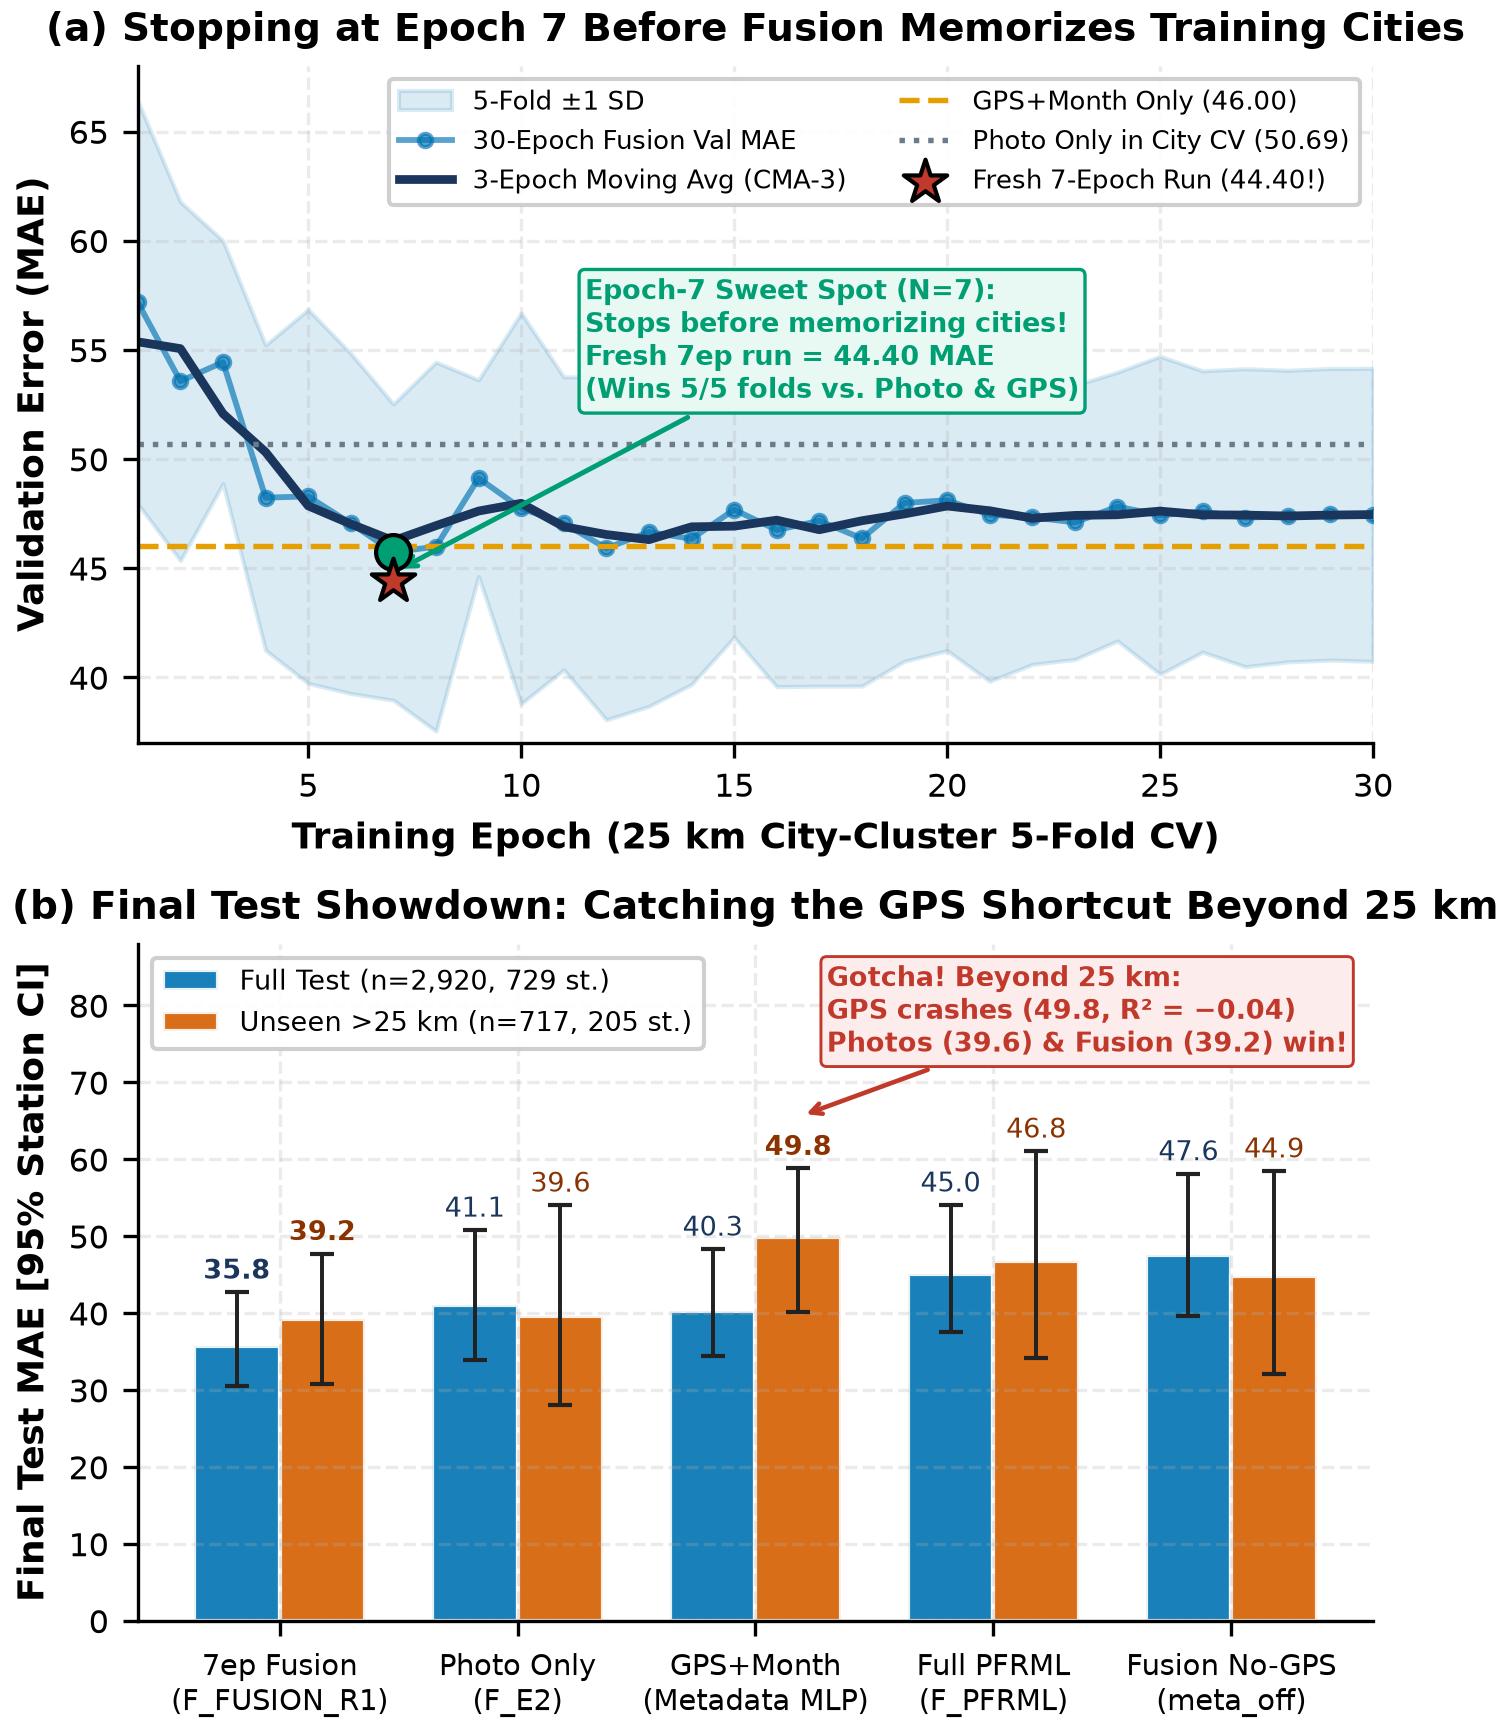
\includegraphics[width=\columnwidth]{figures/story_fig5_gps_cheat_code_and_fusion_win.png}
  \caption{
    \textbf{(a)} Catching the Epoch-7 sweet spot in 25~km city-cluster CV before
    fusion memorizes training cities (fresh 7-epoch run hits 44.40 MAE, winning
    5/5 folds). \textbf{(b)} Final test showdown on all 2,920 test photos vs.\
    717 unseen-region photos $> 25$~km away with 95\% station-bootstrap CIs.
  }
  \label{fig:story_fusion}
\end{figure}

In 5-fold 25~km city-cluster CV (Table~\ref{tab:story_fusion_cv} and
Fig.~\ref{fig:story_fusion}(a)), fusing the prototype-free R1 visual neck again
beats fusing the full PFRML prototype neck ($49.18$ vs.\ $51.68$ MAE at 30
epochs). Watching the per-epoch validation curve of 30-epoch R1 fusion
($p_{\text{drop}} = 0.0$) revealed why 30 epochs is too long: validation MAE
drops rapidly to \textbf{45.74 $\pm$ 6.78 at epoch $N = 7$}
($\text{CMA-3} = 46.26$) before creeping back up to 47.45 by epoch~30 as the
network memorizes training city coordinates. Retraining a fresh \textbf{7-epoch
cosine schedule} achieved \textbf{44.40 $\pm$ 7.30 MAE}, beating both GPS-only
($-1.60 \pm 0.59$, winning \textbf{5/5 folds}) and photo-only ($-6.29 \pm 1.07$,
winning \textbf{5/5 folds}).

On the final one-shot test set
(Tables~\ref{tab:story_final_test}--\ref{tab:story_bootstrap} and
Fig.~\ref{fig:story_fusion}(b)), four takeaways stand out:
\begin{enumerate}
  \item \textbf{Our 7-epoch fusion model (\texttt{F\_FUSION\_R1}) wins overall:}
        It achieves \textbf{35.77~[30.47, 42.72] MAE} ($R^2 = 0.6070$,
        $\text{SRCC} = 0.7941$) on the full test set, significantly beating
        GPS-only by \textbf{$-$4.57~[$-$8.31, $-$1.26] MAE}, photo-only
        \texttt{F\_E2} by \textbf{$-$5.35~[$-$8.62, $-$2.26] MAE}, and full
        PFRML by \textbf{$-$9.26~[$-$12.52, $-$6.06] MAE}.
  \item \textbf{Simple pretrained MobileNetV3-Small (\texttt{F\_E2}) beats full
        PFRML on both test splits:} \texttt{F\_E2} significantly outperforms
        \texttt{F\_PFRML\_full} by \textbf{$-$3.92~[$-$6.27, $-$1.58] MAE} on
        the full test set (41.12 vs.\ 45.04) and by \textbf{$-$7.18~[$-$11.92,
        $-$2.53] MAE} beyond 25~km (39.60 vs.\ 46.79).
  \item \textbf{Beyond 25~km, GPS collapses while vision and fusion hold
        steady:} On \texttt{test\_gt25km} ($n = 717$, 205 stations), GPS-only
        crashes to \textbf{49.84 MAE ($R^2 = -0.0393$)}, whereas photo-only
        \texttt{F\_E2} holds firm at \textbf{39.60 MAE ($R^2 = 0.2747$)} and
        \texttt{F\_FUSION\_R1} achieves \textbf{39.22~[30.85, 47.74] MAE
        ($R^2 = 0.3743$)}, beating GPS-only by \textbf{$-$10.63~[$-$18.78,
        $-$2.59] MAE}.
  \item \textbf{Unplugging GPS at test time (\texttt{meta\_off}) exposes
        continued location reliance:} Zeroing out GPS at evaluation time causes
        \texttt{F\_FUSION\_R1}'s full-test error to jump from 35.77 to
        \textbf{47.56 MAE} (44.88 at $> 25$~km), showing that a shared
        regression layer trained at one learning rate still leans heavily on GPS
        when available.
\end{enumerate}

\subsection{Proven Facts vs.\ Hypotheses and Honest Limitations}
\label{subsec:discussion_limitations}

We explicitly separate what our experiments \textbf{prove} from our
\textbf{hypotheses}:
\begin{itemize}
  \item \textbf{Prototypes:} Our 5-fold CV ladder and test CIs \textit{prove}
        that on global PM25Vision with MobileNetV3-Small, dropping PFRML's
        6-class prototype head (R1, 45.50 CV MAE) and using plain \texttt{F\_E2}
        (41.12 test MAE) beat full PFRML (48.14 CV, 45.04 test). Our
        \textit{hypothesis} is that 6-class AQI classification across
        uncalibrated global cameras is too noisy ($\sim 41\%$ accuracy), so
        cross-entropy overfits after epoch~4 and injects noisy prototype weights
        into regression.
  \item \textbf{City-Cluster CV vs.\ $> 25$~km Test Subset:} In 25~km
        city-cluster CV, GPS-only beat photo-only (46.00 vs.\ 50.69), whereas on
        \texttt{test\_gt25km} photo-only beat GPS-only by 10.24 points (39.60
        vs.\ 49.84, 95\% CI $[-20.50, +0.86]$ slightly crossing zero). Our
        \textit{hypothesis} is that the 205 remote test stations have fewer
        extreme $> 300$ AQI episodes than the training folds (where the Blind
        Median Guess gets 56.60 MAE on \texttt{test\_gt25km} vs.\ 66.14 in
        city-cluster CV).
\end{itemize}

\textbf{Limitations:} (1) All runs used a single random seed
($\text{seed} = 42$) across $n = 5$ folds (where a paired Wilcoxon test has a
mathematical floor of $p_{\min} = 0.0625 > 0.05$); (2) picking $N = 7$ epochs
from the 30-epoch CV curve introduces mild CV selection optimism (verified
independently on the one-shot test set); (3) \texttt{test\_gt25km} has only 205
stations (wide 17--26 MAE CIs and $\text{TailF1} = 0.0000$ across all models);
(4) we substituted a 2M-parameter MobileNetV3-Small spine for Paper~1's
115M-parameter ResNet-50 + ViT; (5) Apple Silicon \texttt{mps} training has
minor floating-point hardware variance; and (6) future work should test smaller
learning rates on the GPS branch or distance-based ensembling of standalone
photo and GPS models.

\section{Conclusion}
\label{sec:conclusion}

Our journey predicting global air quality on the cleaned PM25Vision benchmark
(8,176 training photos across 2,527 stations; 2,920 test photos across 729
stations, including 717 unseen-region photos $> 25$~km away) taught us that when
an ambitious model flops (like our initial 66.56 MAE MDNet-T + PFRML run), a
controlled multi-model investigation is the best way forward:
\begin{itemize}
  \item \textbf{Q1 (Audit shortcuts first):} A 5-input GPS + month MLP gets
        40.34 test MAE ($R^2 = 0.4982$) near training cities, but collapses
        beyond 25~km (49.84 MAE, $R^2 = -0.0393$).
  \item \textbf{Q2 (Pretraining wins):} ImageNet pretraining lowers 5-fold
        vision MAE by 7.6 to 9.2 points ($44.05\text{--}45.66$ vs.\
        $53.27\text{--}53.29$), and our 1.04M-parameter MobileNetV3-S + MD-Neck
        adaptation (\texttt{E3b}) reaches $44.92 \pm 8.54$ MAE.
  \item \textbf{Q3 (Simpler regression beats 6-class prototypes):} PFRML's
        multi-stage neck without prototypes (R1, $45.50 \pm 8.64$) beats every
        prototype variant (R2, $48.14$; Eq.~5, $48.04$), and plain
        \texttt{F\_E2} significantly beats \texttt{F\_PFRML\_full} on both test
        splits ($-3.92$ full test; $-7.18$ at $> 25$~km).
  \item \textbf{Q4 (Early-stopped fusion wins overall):} Fusing the
        prototype-free R1 visual spine with GPS/month metadata and stopping at
        epoch $N = 7$ (\texttt{F\_FUSION\_R1}) achieves our lowest test error on
        both the full test set (\textbf{35.77~[30.47, 42.72] MAE},
        $R^2 = 0.6070$) and unseen regions $> 25$~km away (\textbf{39.22~[30.85,
        47.74] MAE}, $R^2 = 0.3743$).
\end{itemize}

\textbf{Reproducibility:} Executed at commit \texttt{fd7bea3}
($\text{seed} = 42$) on an Apple M5 Pro MacBook Pro (24~GB RAM, Python 3.14.6,
PyTorch 2.14.1 \texttt{mps}, \texttt{fp32}); all tables and figures regenerate
offline from \texttt{results/}.

\bibliographystyle{IEEEtran}
\bibliography{references}

\end{document}
